%!TEX root = Manuscript.tex

\chapter{Rough co-registration}
\label{chap:intro}
\minitoc

\section{Introduction}
The goal of rough co-registration is establish a transformation model between different epochs to guide the subsequent precise matching step. Minimum matches between different epochs are required, depending on the model type:\\
\begin{enumerate}
    \item 2D similarity transformation model, which requires at least 2 matches for each inter-epoch image pair to solve 4 parameters;
    \item Homography transformation model, which requires at least 4 matches for each inter-epoch image pair to solve 8 parameters;
    \item 3D Helmert transformation model, which requires at least 3 matches for the whole block to solve 7 parameters.
\end{enumerate}
Generally, each inter-epoch image pair would be matched, followed by a RANSAC routine to recover the best transformation model.
The most critical target is to get reliable matches, instead of obtaining accurately localized ones.
Since multi-epoch images often demonstrate different appearances due to scene changes and heterogeneous acquisition conditions, we come up with 2 ideas in order to improve the matching robustness:\\
\begin{enumerate}
    \item Instead of building transformation models (2D similarity or homography) for each inter-epoch image pair that might contradict each other, it is better to build a 3D Helmert transformation model which is globally consistent over the whole block.
    \item Take 3D geometry into consideration to boost the matching performance.
\end{enumerate}
Based on these ideas, we attempted 2 strategies to match different epochs:\\
\begin{enumerate}
    \item Match each inter-epoch image pair, followed by projecting the matches onto ground to build globally consistent transformation model.
    \item Generate orthophoto or DSM for each epoch, and match orthophoto/DSM pairs instead of matching the inter-epoch image pairs, followed by RANSAC based on 2D similarity transformation model to remove outliers, and build a 3D Helmert transformation model between epochs by projecting inlier mathces to ground.
\end{enumerate}

%\subsection{Motivation}
%\subsection{Contribution}

\section{Methodology}
%Our goal is to improve robustness by building globally consistent transformation model over the whole block.
%In order to achieve this goal, we exploded 2 strategies:
%(1) matching each potential image pair followed with global filtering based on 3D RANSAC;\\
%(2) get a global image for each epoch first (DSM or orthophoto), apply matching and 2D RANSAC.\\
%零碎匹配,整体inlier
%整体匹配
Our methods expect the images accompanied with focal lengths and physical sensor sizes, which are usually available. The images are resampled to the geometry of the fiducial marks prior to processing. For the sake of simplicity, only 2 epochs are present in our processing flows, however, it can be easily extended to more epochs.
\par
We adopt the following naming conventions:\\
\begin{enumerate}
    \item Images acquired in \textit{epoch$_1$} and \textit{epoch$_2$} are denoted as $I^{e_1}$ and $I^{e_2}$;
    \item Orientations of \textit{epoch$_1$} and \textit{epoch$_2$} are denoted as $O^{e_1}$ and $O^{e_2}$; 
    \item Mean elevation plane of the Ground in \textit{epoch$_1$} and \textit{epoch$_2$} are denoted as $G^{e_1}$ and $G^{e_2}$;
    \item Orthophotos of \textit{epoch$_1$} and \textit{epoch$_2$} are denoted as $Op^{e_1}$ and $Op^{e_2}$; 
    \item DSMs of \textit{epoch$_1$} and \textit{epoch$_2$} are denoted as $D^{e_1}$ and $D^{e_2}$.
\end{enumerate}
\par
Before matching different epochs, we process each epoch individually to recover the relative orientation within the same epoch. It is a standard photogrammetry or SfM pipeline and can be accomplished with lots of solutions (e.g. MicMac~\cite{deseilligny2011apero}, COLMAP~\cite{schonberger2016structure}, {OpenMVG~\cite{openMVG}, Theia~\cite{theia}, etc.}). The solution used in our experiment is MicMac. It is performed within each \textit{epoch$_i$} individually as follows:
\begin{enumerate}
\item Extract intra-epoch correspondences between images $I^{e_i}$ with SIFT ~\cite{lowe2004distinctive};
\item Compute interior and relative orientations ({$O_{ini}^{e_i}$}) with the sequential SfM;
\item Based on image orientations $O_{ini}^{e_i}$, perform semi-global dense matching~\cite{mpd:06:sgm} {between images $I^{e_i}$} to get {DSM ($D_{ini}^{e_i}$) in their arbitrary coordinate frames.}
\item Orthorectify the images to get orthophotos ($Op_{ini}^{e_i}$).
%\item Project the images onto mean elevation plane ($G_{ini}^{e_i}$) get orthophotos ($Op_{ini}^{e_i}$).
\end{enumerate}

Two different strategies are provided to perform the rough co-registration. The pipelines will be elaborated in the following sections. 
\par
Please notice our pipelines are generic, different feature matching methods can be readily applied in them. At present we use either SIFT or SuperGlue to test our pipeline as they are currently \textit{state-of-the-art}, but they can be replaced when better matching methods appear in the future.\\
\subsection{Strategy 1: Matching image pairs}
%\subsection{Strategy 1: global filtering}
%CoReg-R3D
The workflow of matching image pairs strategy is displayed in Figure~\ref{WorkflowImgPair}.\\
We introduce \textit{4 rotation hypotheses} when feature matching method that is not invariant to rotations lager than 45$^\circ$ (e.g. SuperGlue) is applied. It works as follows (cf. Figure~\ref{WorkflowImgPair}(b)): 
\begin{enumerate}
    \item Rotate the secondary image by 90$^{\circ}$ four times;
    \item Match each rotated image with the master image;
    \item Keep the hypothesis with the largest number of matches.
\end{enumerate}
The \textit{4 rotation hypotheses} would not be applied when rotation invariant matching method (e.g. SIFT) is adopted.
\par
Assuming the numbers of images in \textit{epoch$_1$} and \textit{epoch$_2$} are P and Q individually, the matching image pairs strategy works as follows:\\
\begin{enumerate}
    \item Match P$\times$Q image pairs respectively (with or without \textit{4 rotation hypotheses}, depending on whether the matching method is rotation invariant), giving rise to P$\times$Q sets of matches $M({\mathbf{K}^{e_1},\mathbf{K}^{e_2}})$ ($\mathbf{K}^{e_i}$ represents keypoints in image $I^{e_i}$).
    \item Project matches $M({\mathbf{K}^{e_1},\mathbf{K}^{e_2}})$ of each image pair onto ground, resulting in one set of matches $M({\mathbf{KG}^{e_1},\mathbf{KG}^{e_2}})$ ($\mathbf{KG}^{e_i}$ represents keypoints on ground $G^{e_i}$).
    \item Sample matches $M({\mathbf{KG}^{e_1},\mathbf{KG}^{e_2}})$ iteratively to compute the 3D Helmert transformation RANSAC model:
\begin{equation}
\left [ \begin{array}{c}
{KG}_x^{e_2}\\
{KG}_y^{e_2}\\
{KG}_z^{e_2}
\end{array}
\right ] =\lambda \cdot \mathbf{R} \cdot {\left [ \begin{array}{c}
    {KG}_x^{e_1}\\
    {KG}_y^{e_1}\\
    {KG}_z^{e_1}
    \end{array}
    \right ]} + \left [ \begin{array}{c}
\Delta_x\\
\Delta_y\\
\Delta_z
\end{array}
\right ]. \label{eq:2DSim}
\end{equation}
    
%   \begin{equation*}
%       {KG_i^{e_2}} = \lambda \cdot \mathbf{R} \cdot {KG_i^{e_1}} + \mathbf{T} , \quad i \in [1,3] \label{eq:3Dsim}
%   \end{equation*}
where $\lambda$ is the scale factor, $\mathbf{R}$ is the rotation matrix and $\left [ \begin{array}{c}
    \Delta_x, \Delta_y, \Delta_z
\end{array}
\right ]$ $^{^T}$ is the translation vector.
We set the number of RANSAC iterations to 1000, and consider matches within $T_r$ of its predicted position as inliers. In our experiment, {$T_r$ was set to 50m.}
    % to find the best 3D Helmert transformation model.
\end{enumerate}

\begin{figure*}[htbp]
    \begin{center}
        \subfigure[Workflow]{
    \begin{minipage}[t]{1\linewidth}
        \centering
        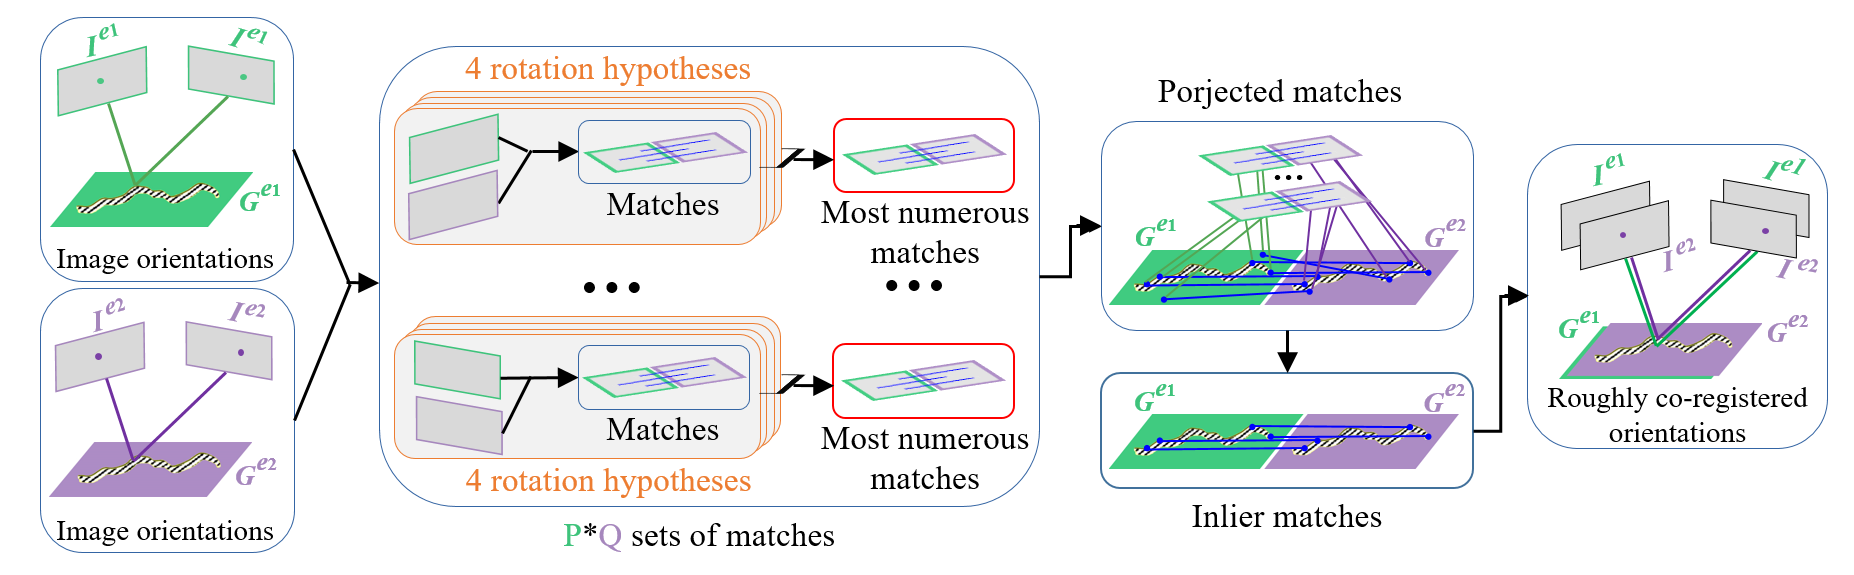
\includegraphics[width=1\columnwidth]{images/Chapitre3/R3D.png}
    \end{minipage}%
}
        \subfigure[Four rotation hypotheses]{
    \begin{minipage}[t]{0.8\linewidth}
        \centering
        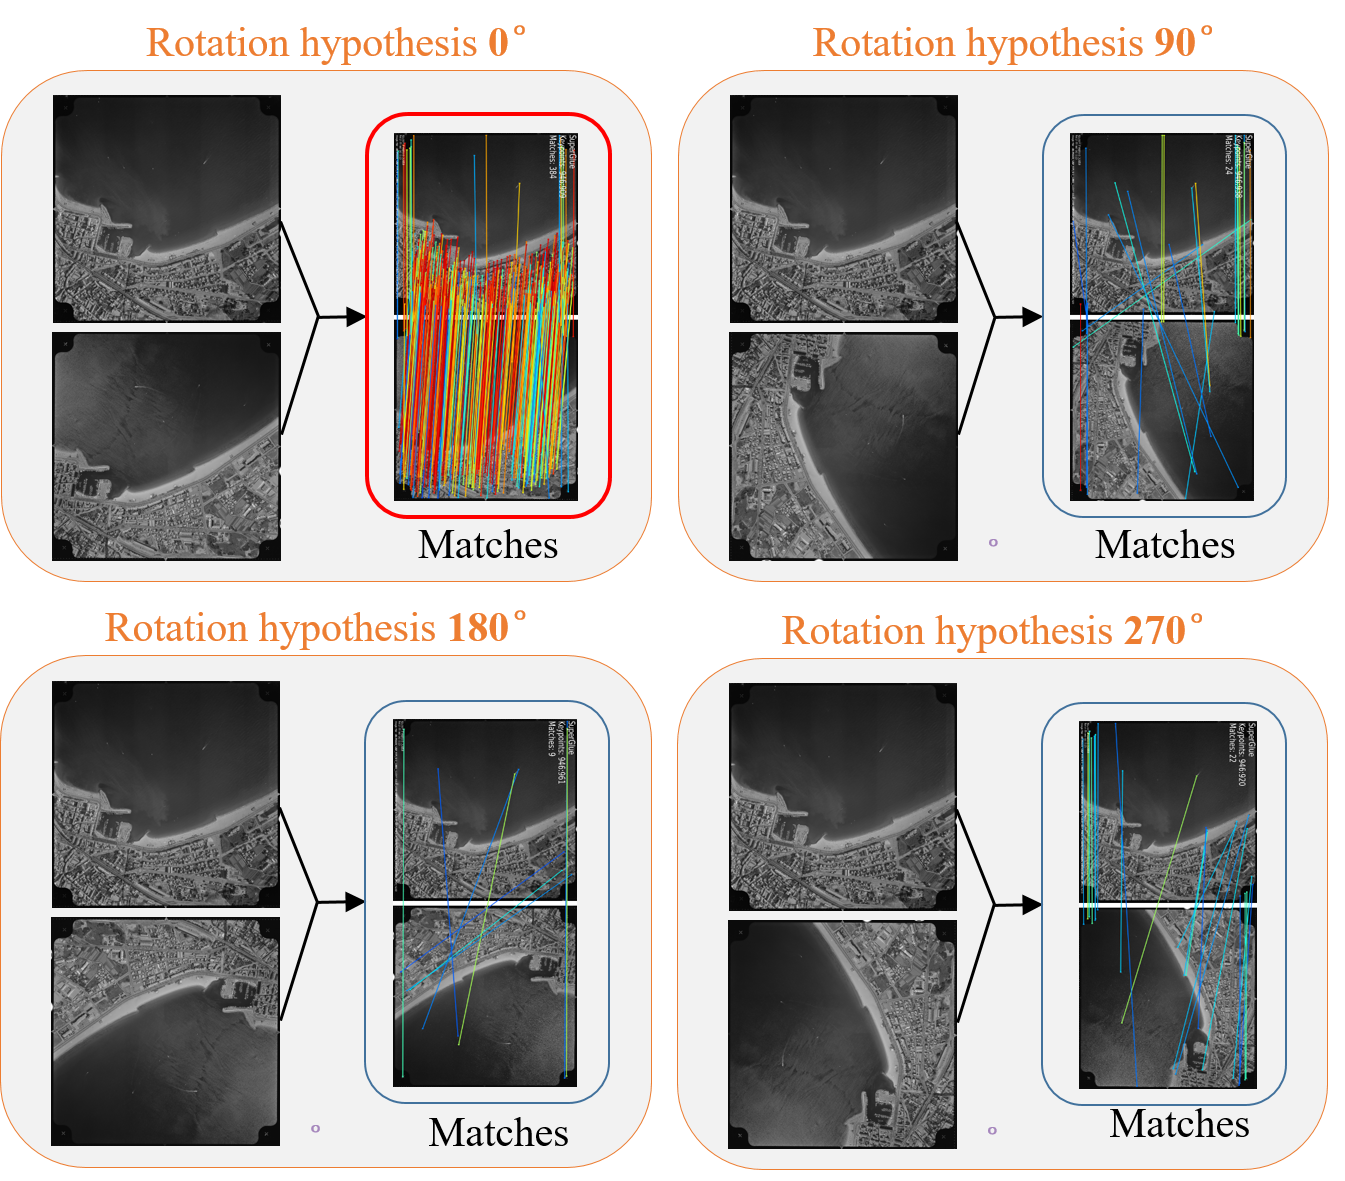
\includegraphics[width=0.8\columnwidth]{images/Chapitre3/R3D-RotHyp.png}
    \end{minipage}%
}
        \caption{Rough co-registration by matching image pairs. (a) Workflow. Each inter-epoch image pair is matched (with 4 rotation hypotheses which are explained in (b), if the matching method is not rotation invariant), followed by projecting the matches onto ground to find the globally consistent inliers. (b) Four rotation hypotheses. We rotate the secondary image by 90 $^\circ$ four times to match with master image and keep the best one with the largest number of matches (red rectangle).}
        \label{WorkflowImgPair}
    \end{center}
\end{figure*}

%\begin{figure*}[htbp]
%    \begin{center}
%        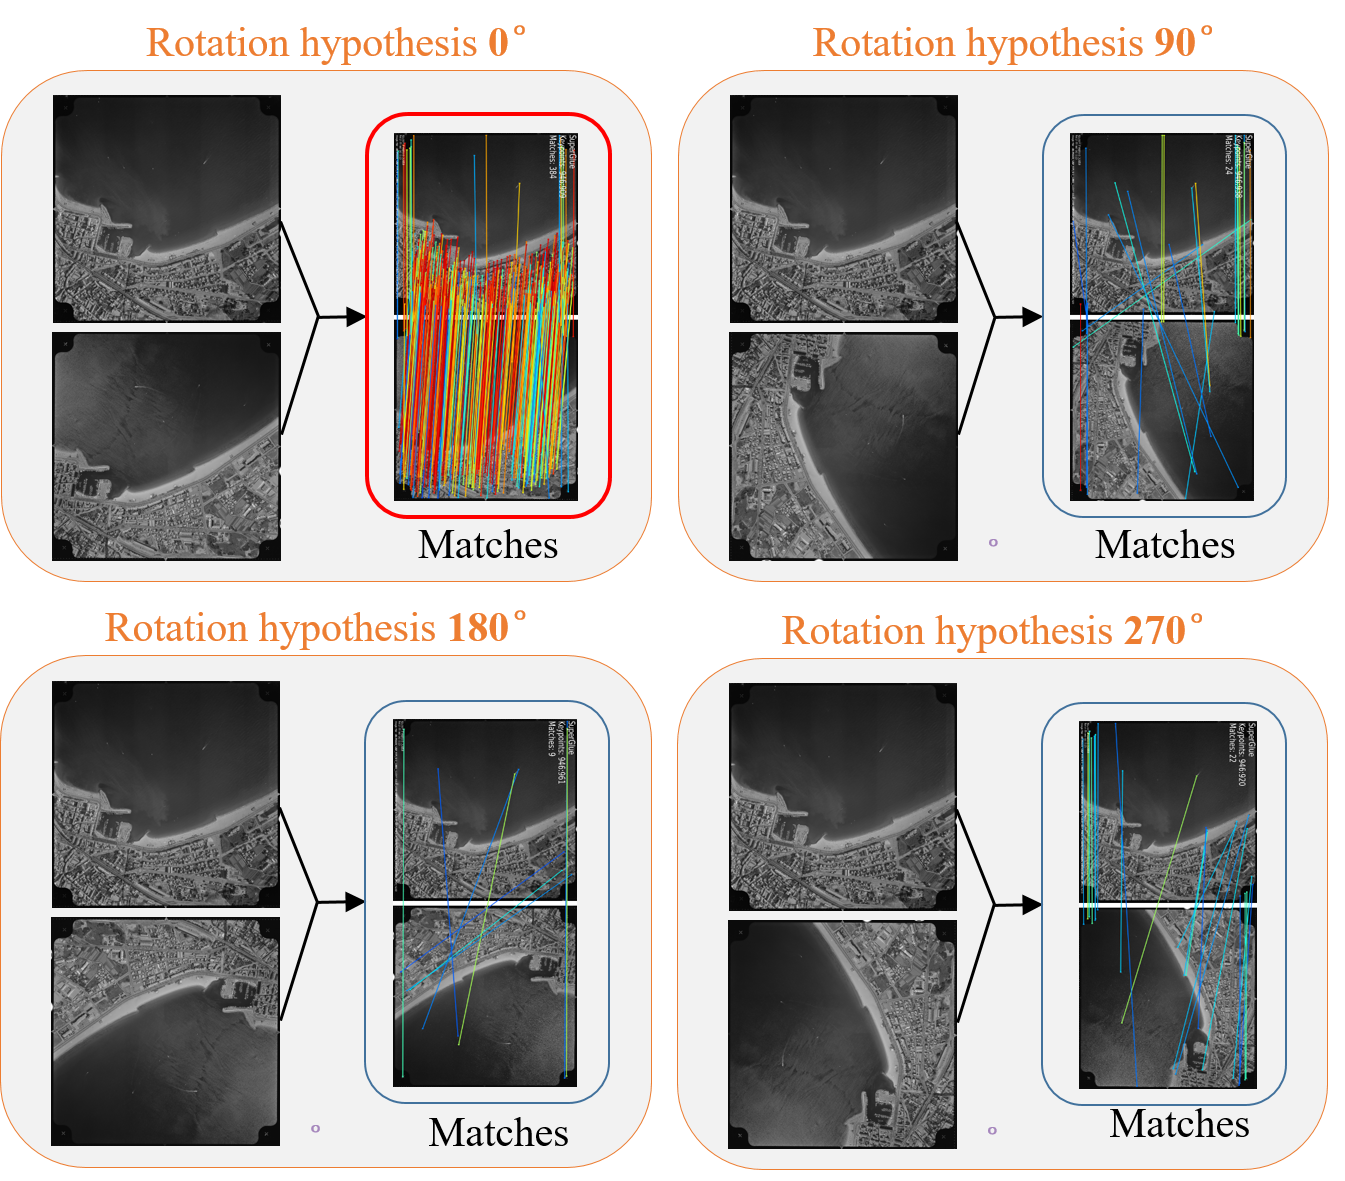
\includegraphics[width=0.8\columnwidth]{images/Chapitre3/R3D-RotHyp.png}
%        \caption{4 rotation hypotheses of matching image pairs.}
%        \label{Flow-process diagram}
%    \end{center}
%\end{figure*}

%\subsubsection{SIFT}
%\subsubsection{SuperGlue}
\subsection{Strategy 2: Matching Orthophotos/DSMs}
%\subsection{trategy 2: global matching}
Another strategy is to match orthophotos or DSMs, the workflows are displayed in Figure~\ref{WorkflowOrtho} and Figure~\ref{WorkflowDSM} individually. Different than matching P$\times$Q image pairs, we only need to match a pair of DSMs/orthophotos.
Orthophotos are by nature RGB images, therefore feature matching methods can be applied on them directly. Conversely, DSMs are 2.5D rasters recorded in floating-point format, they should be converted beforehand to [0–255] range grayscale images.
\par
\begin{figure*}[htbp]
    \begin{center}
        \subfigure[Workflow]{
            \begin{minipage}[t]{1\linewidth}
                \centering
                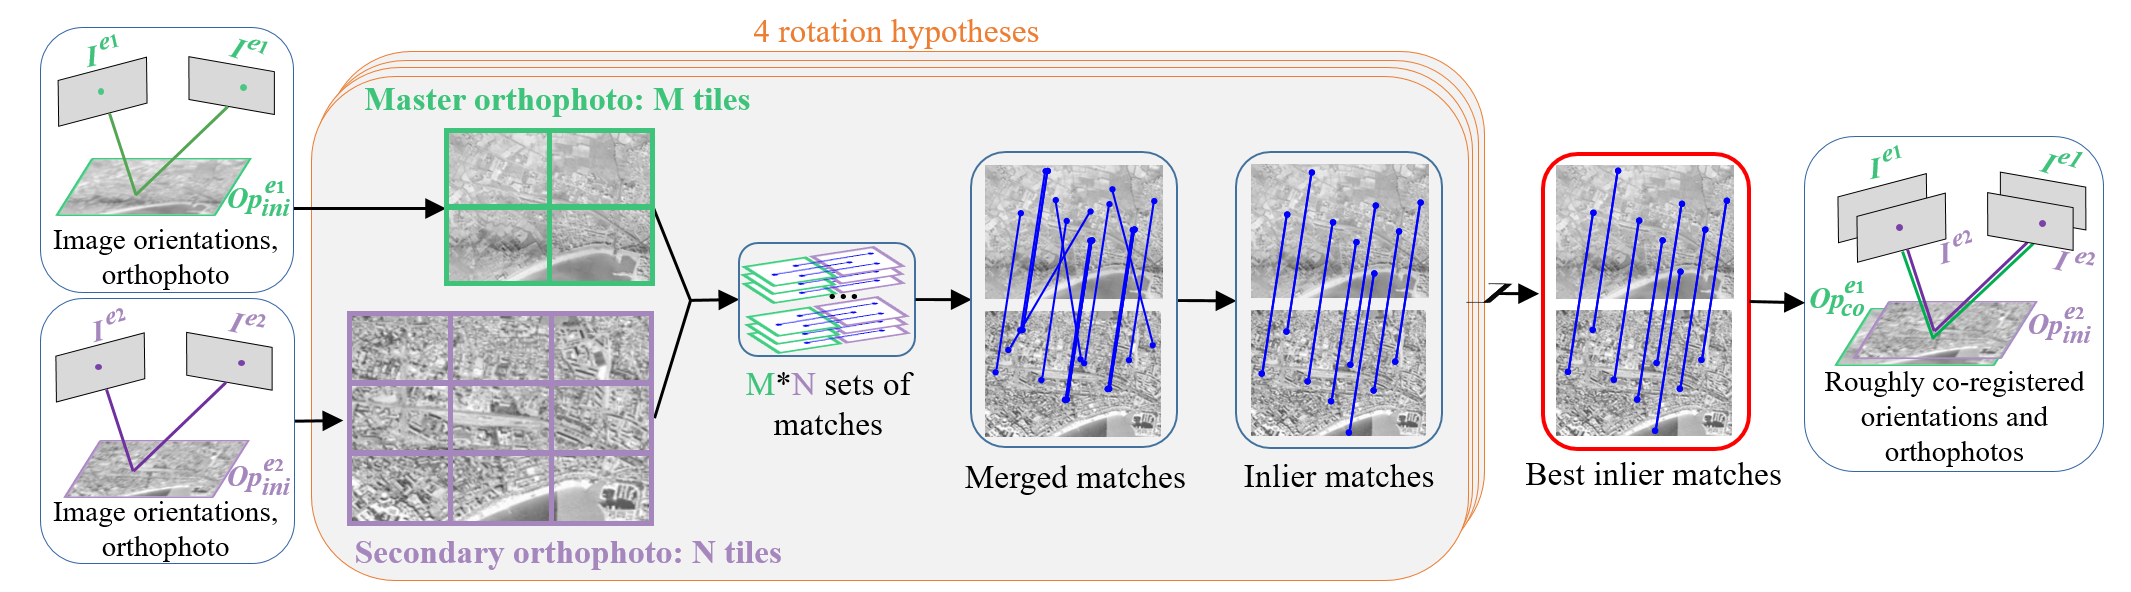
\includegraphics[width=1\columnwidth]{images/Chapitre3/ortho.png}
            \end{minipage}%
        }
        \subfigure[Four rotation hypotheses combined with tiling scheme]{
            \begin{minipage}[t]{1\linewidth}
                \centering
                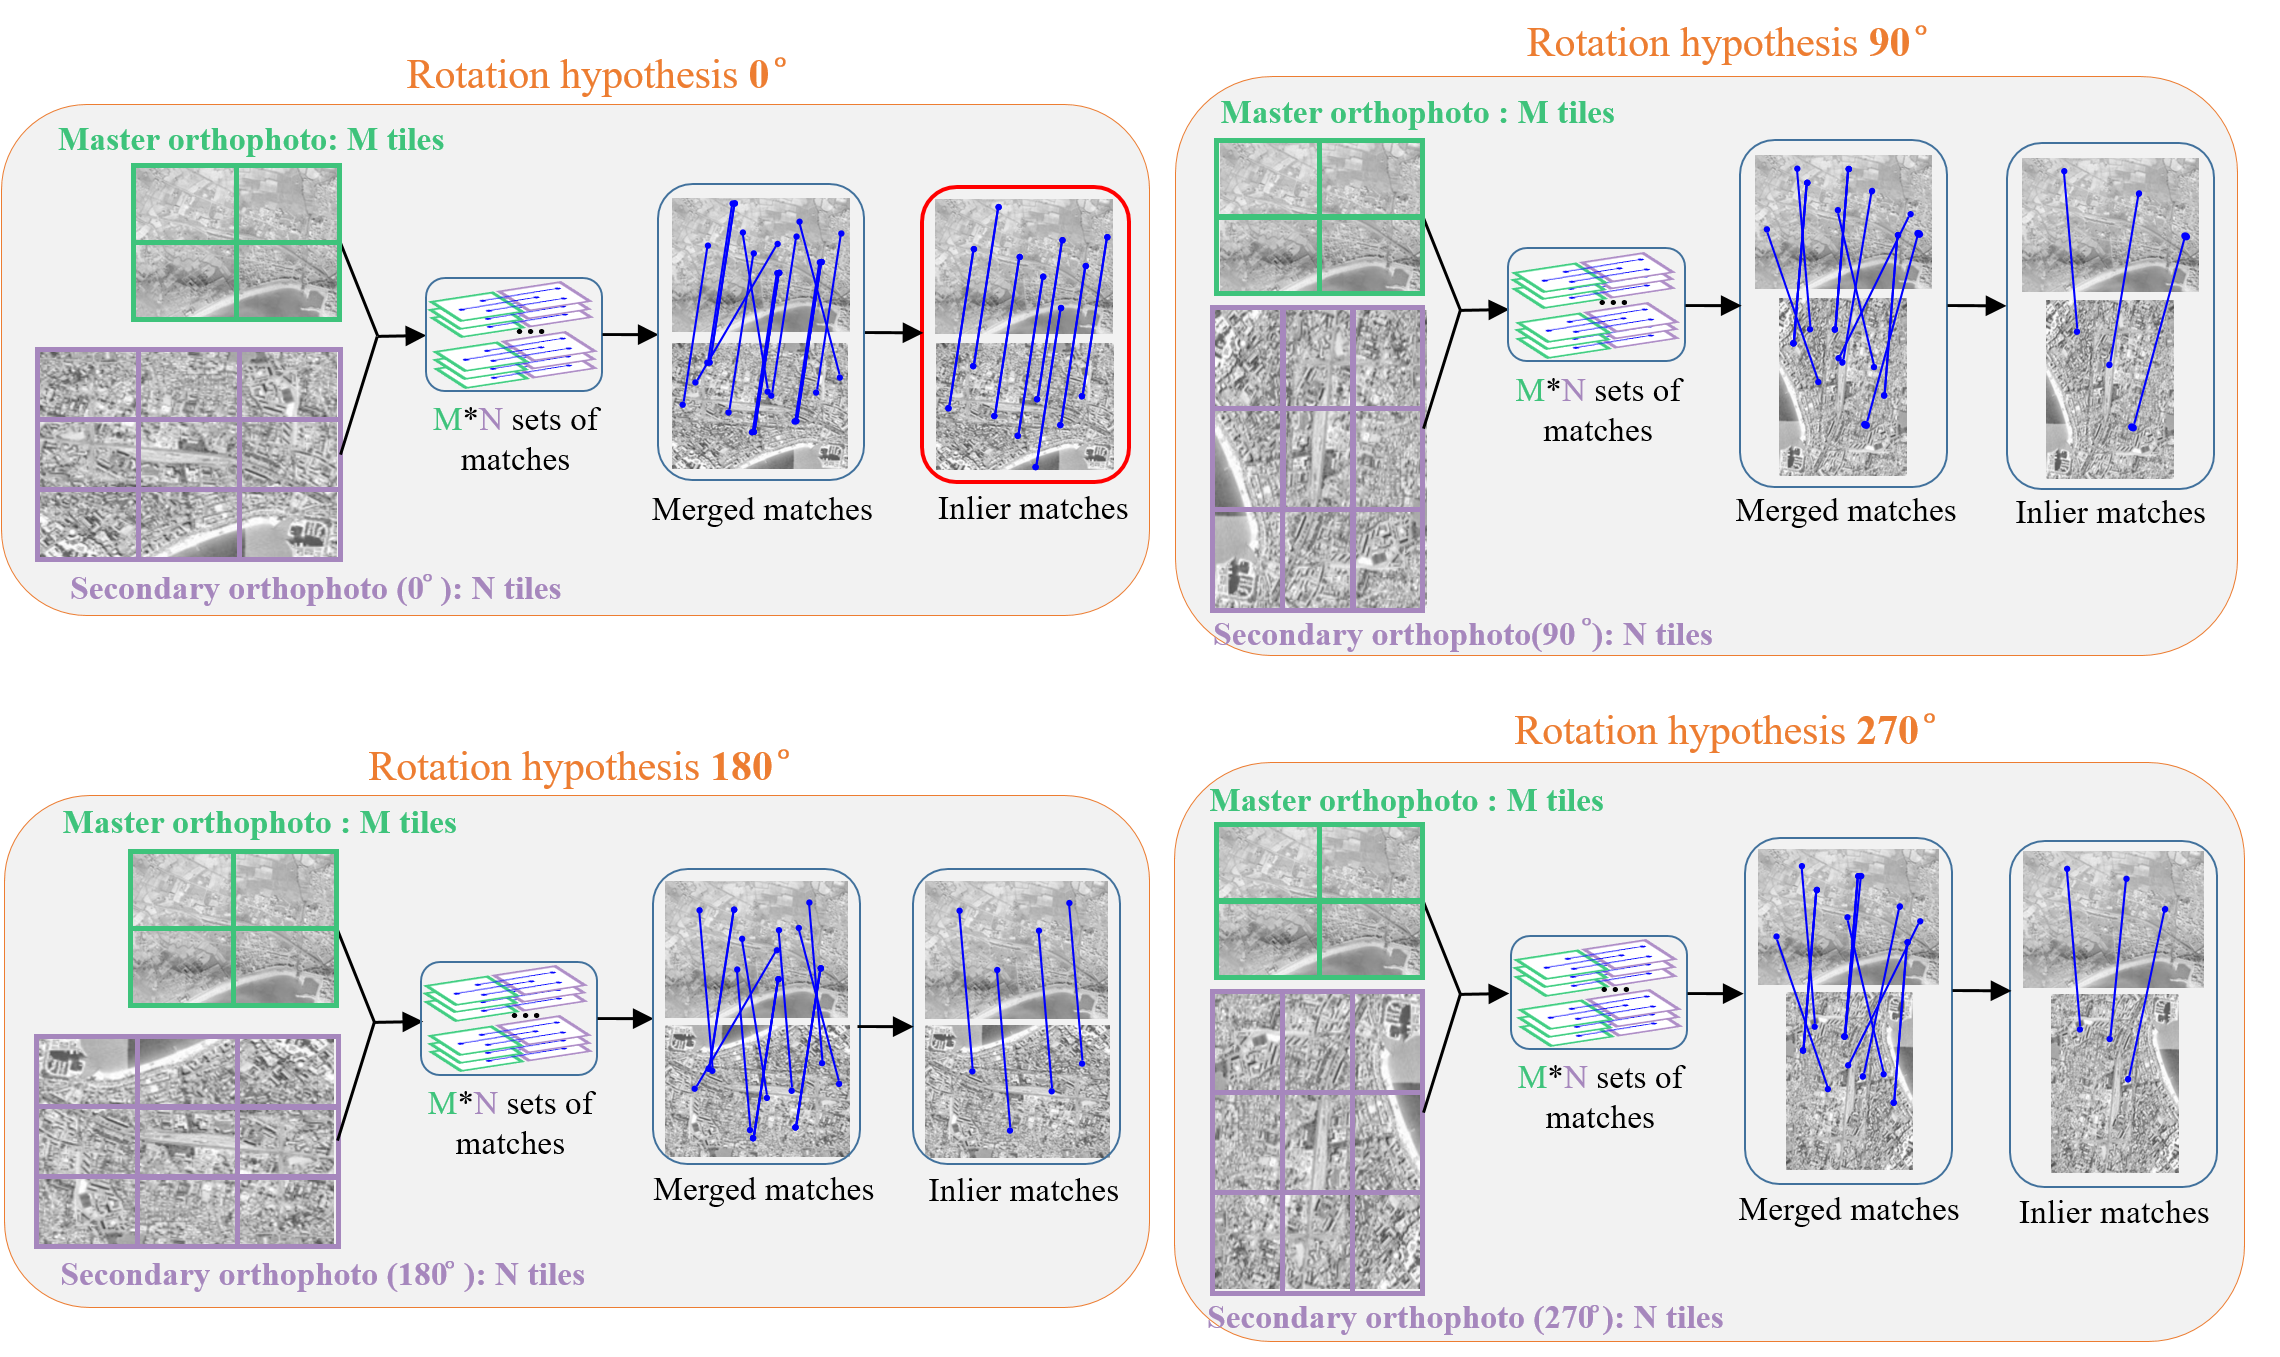
\includegraphics[width=1\columnwidth]{images/Chapitre3/ortho-RotHyp.png}
            \end{minipage}%
        }
        \caption{Rough co-registration by matching orthophotos. (a) Workflow. Orthophotos are matched (with 4 rotation hypotheses combined with tiling scheme which are explained in (b), if the matching method is not rotation invariant), followed by projecting the inlier matches onto ground to build 3D Helmert transformation model. (b) Four rotation hypotheses combined with tiling scheme. We rotate the secondary orthophoto by 90 $^\circ$ four times to match with master orthophoto and keep the best one with the largest number of RANSAC inliers (red rectangle). Tiling scheme is applied during each hypothesis, with both orthophotos croped into tiles followed by matching all the tile pairs and merging the matches.}
        \label{WorkflowOrtho}
    \end{center}
\end{figure*}

%\begin{figure*}[htbp]
%    \begin{center}
%        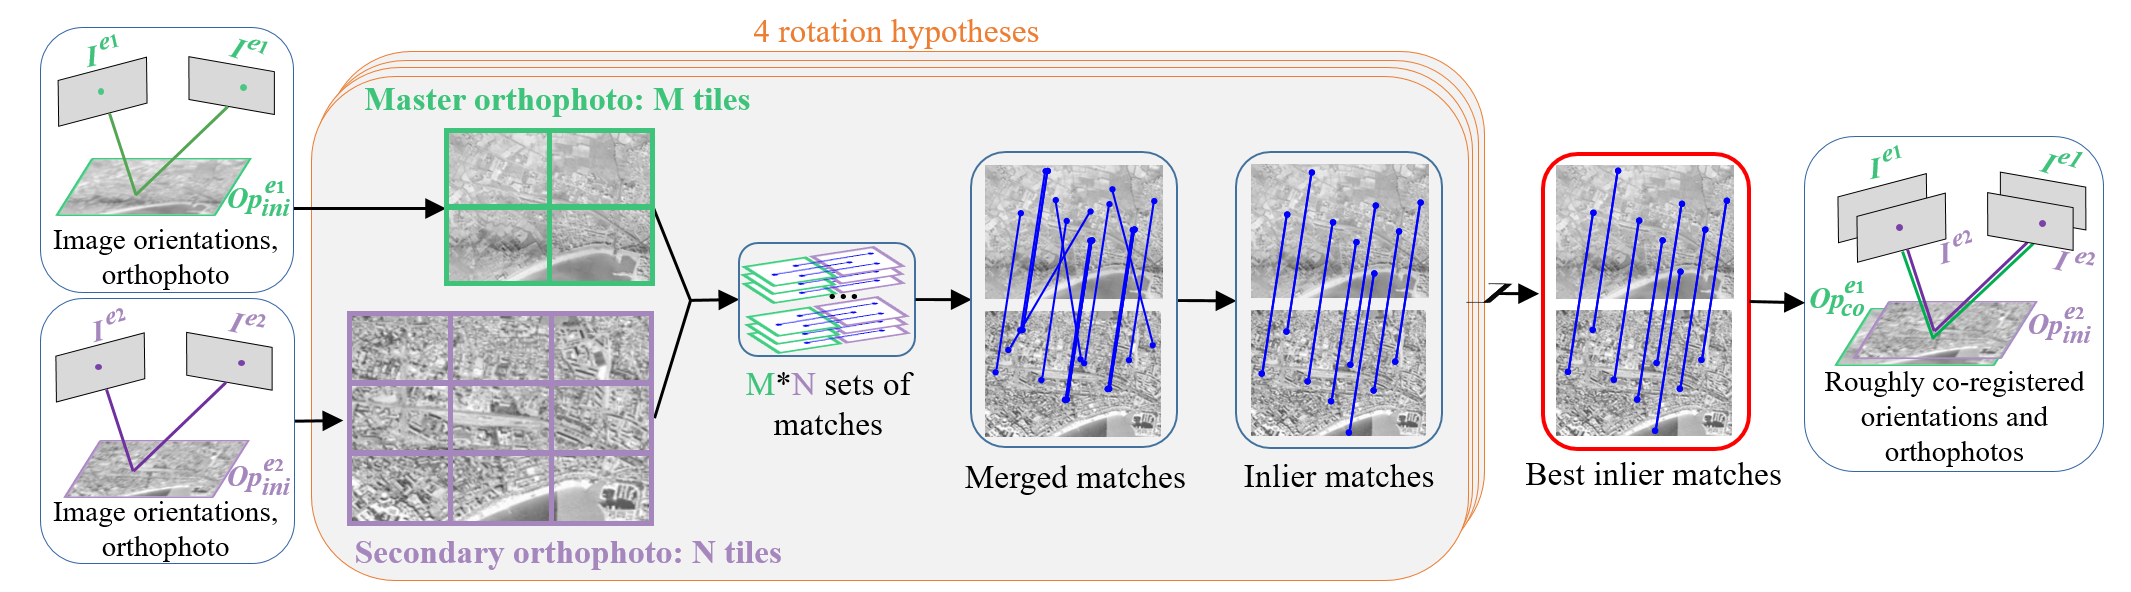
\includegraphics[width=1\columnwidth]{images/Chapitre3/ortho.png}
%        \caption{Rough co-registration by matching orthophotos.}
%        \label{Flow-process diagram}
%    \end{center}
%\end{figure*}
%
%\begin{figure*}[htbp]
%    \begin{center}
%        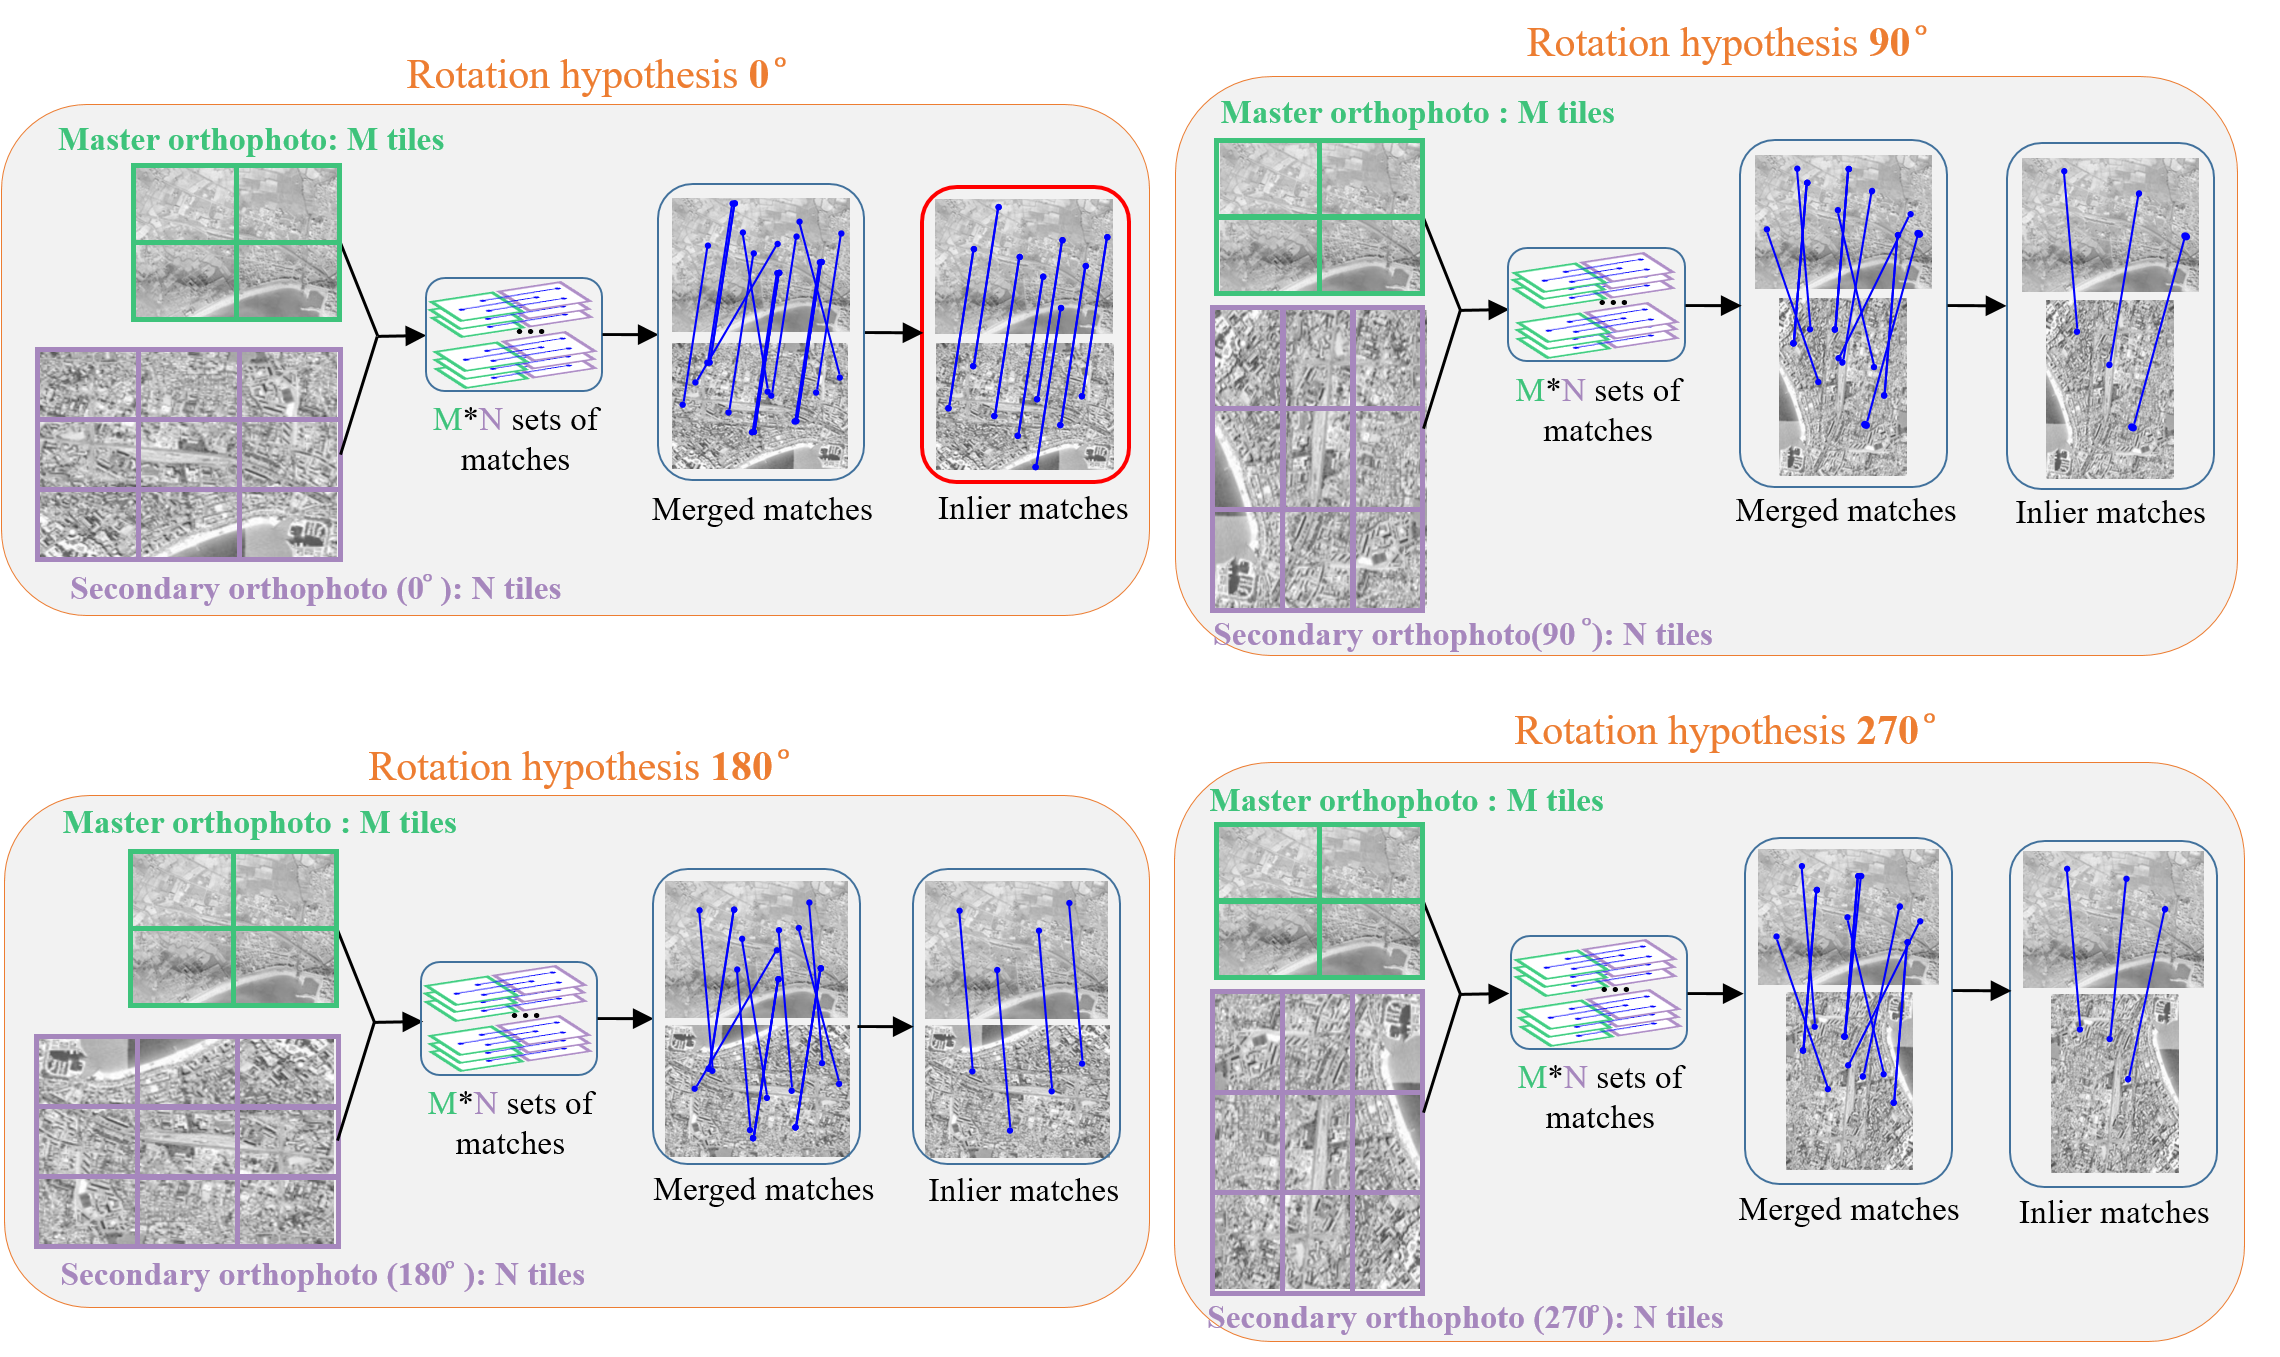
\includegraphics[width=0.8\columnwidth]{images/Chapitre3/ortho-RotHyp.png}
%        \caption{4 rotation hypotheses of matching orthophotos.}
%        \label{Flow-process diagram}
%    \end{center}
%\end{figure*}

%%%%%%%%%%%%%%%%%%%%%%%%%%%%%%

\begin{figure*}[htbp]
    \begin{center}
        \subfigure[Workflow]{
            \begin{minipage}[t]{1\linewidth}
                \centering
                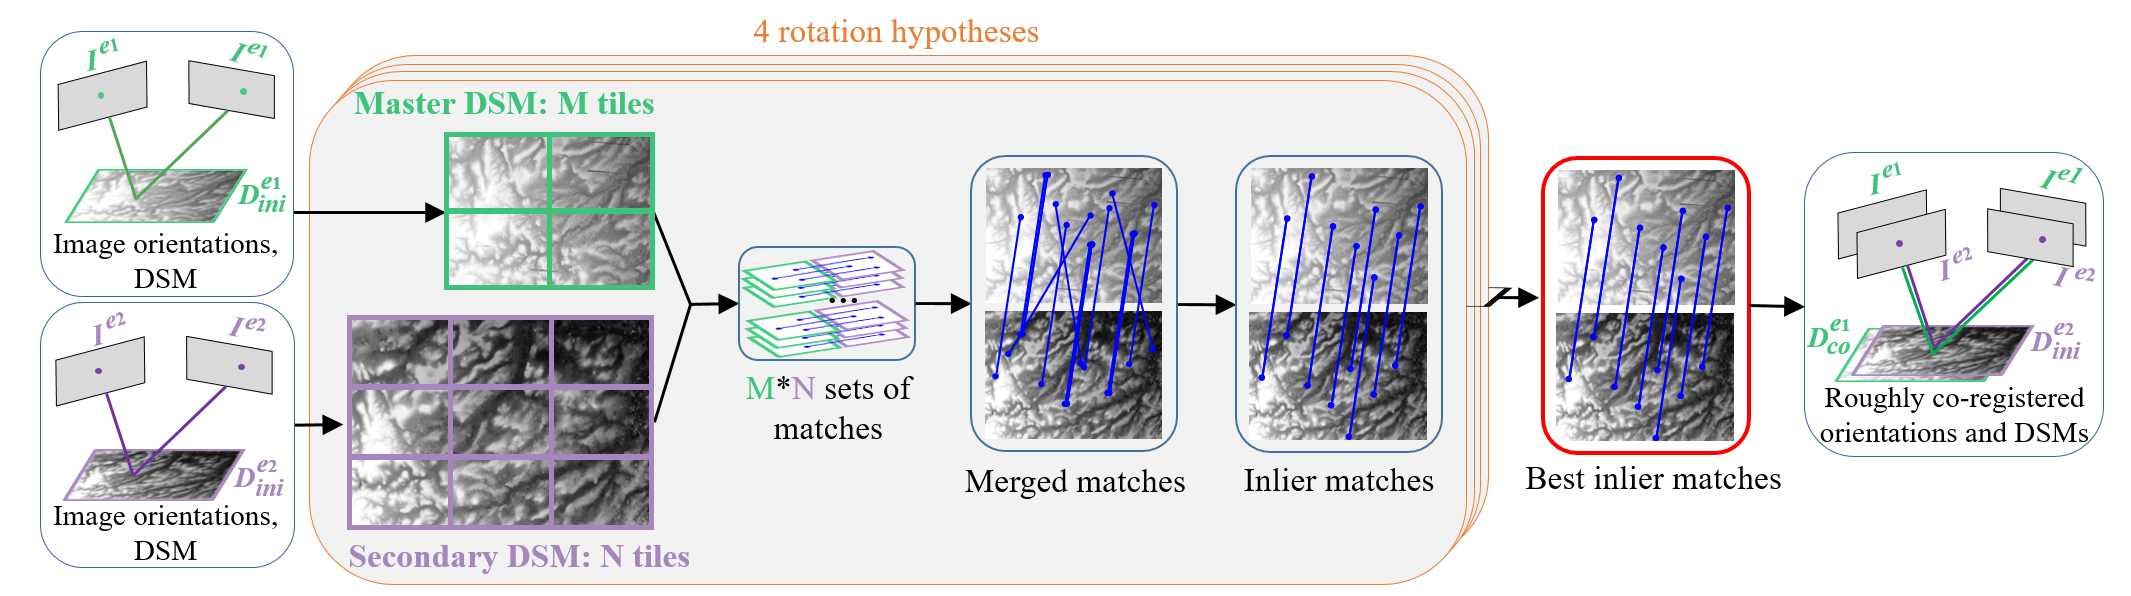
\includegraphics[width=1\columnwidth]{images/Chapitre3/dsm.png}
            \end{minipage}%
        }
        \subfigure[Four rotation hypotheses combined with tiling scheme]{
            \begin{minipage}[t]{1\linewidth}
                \centering
                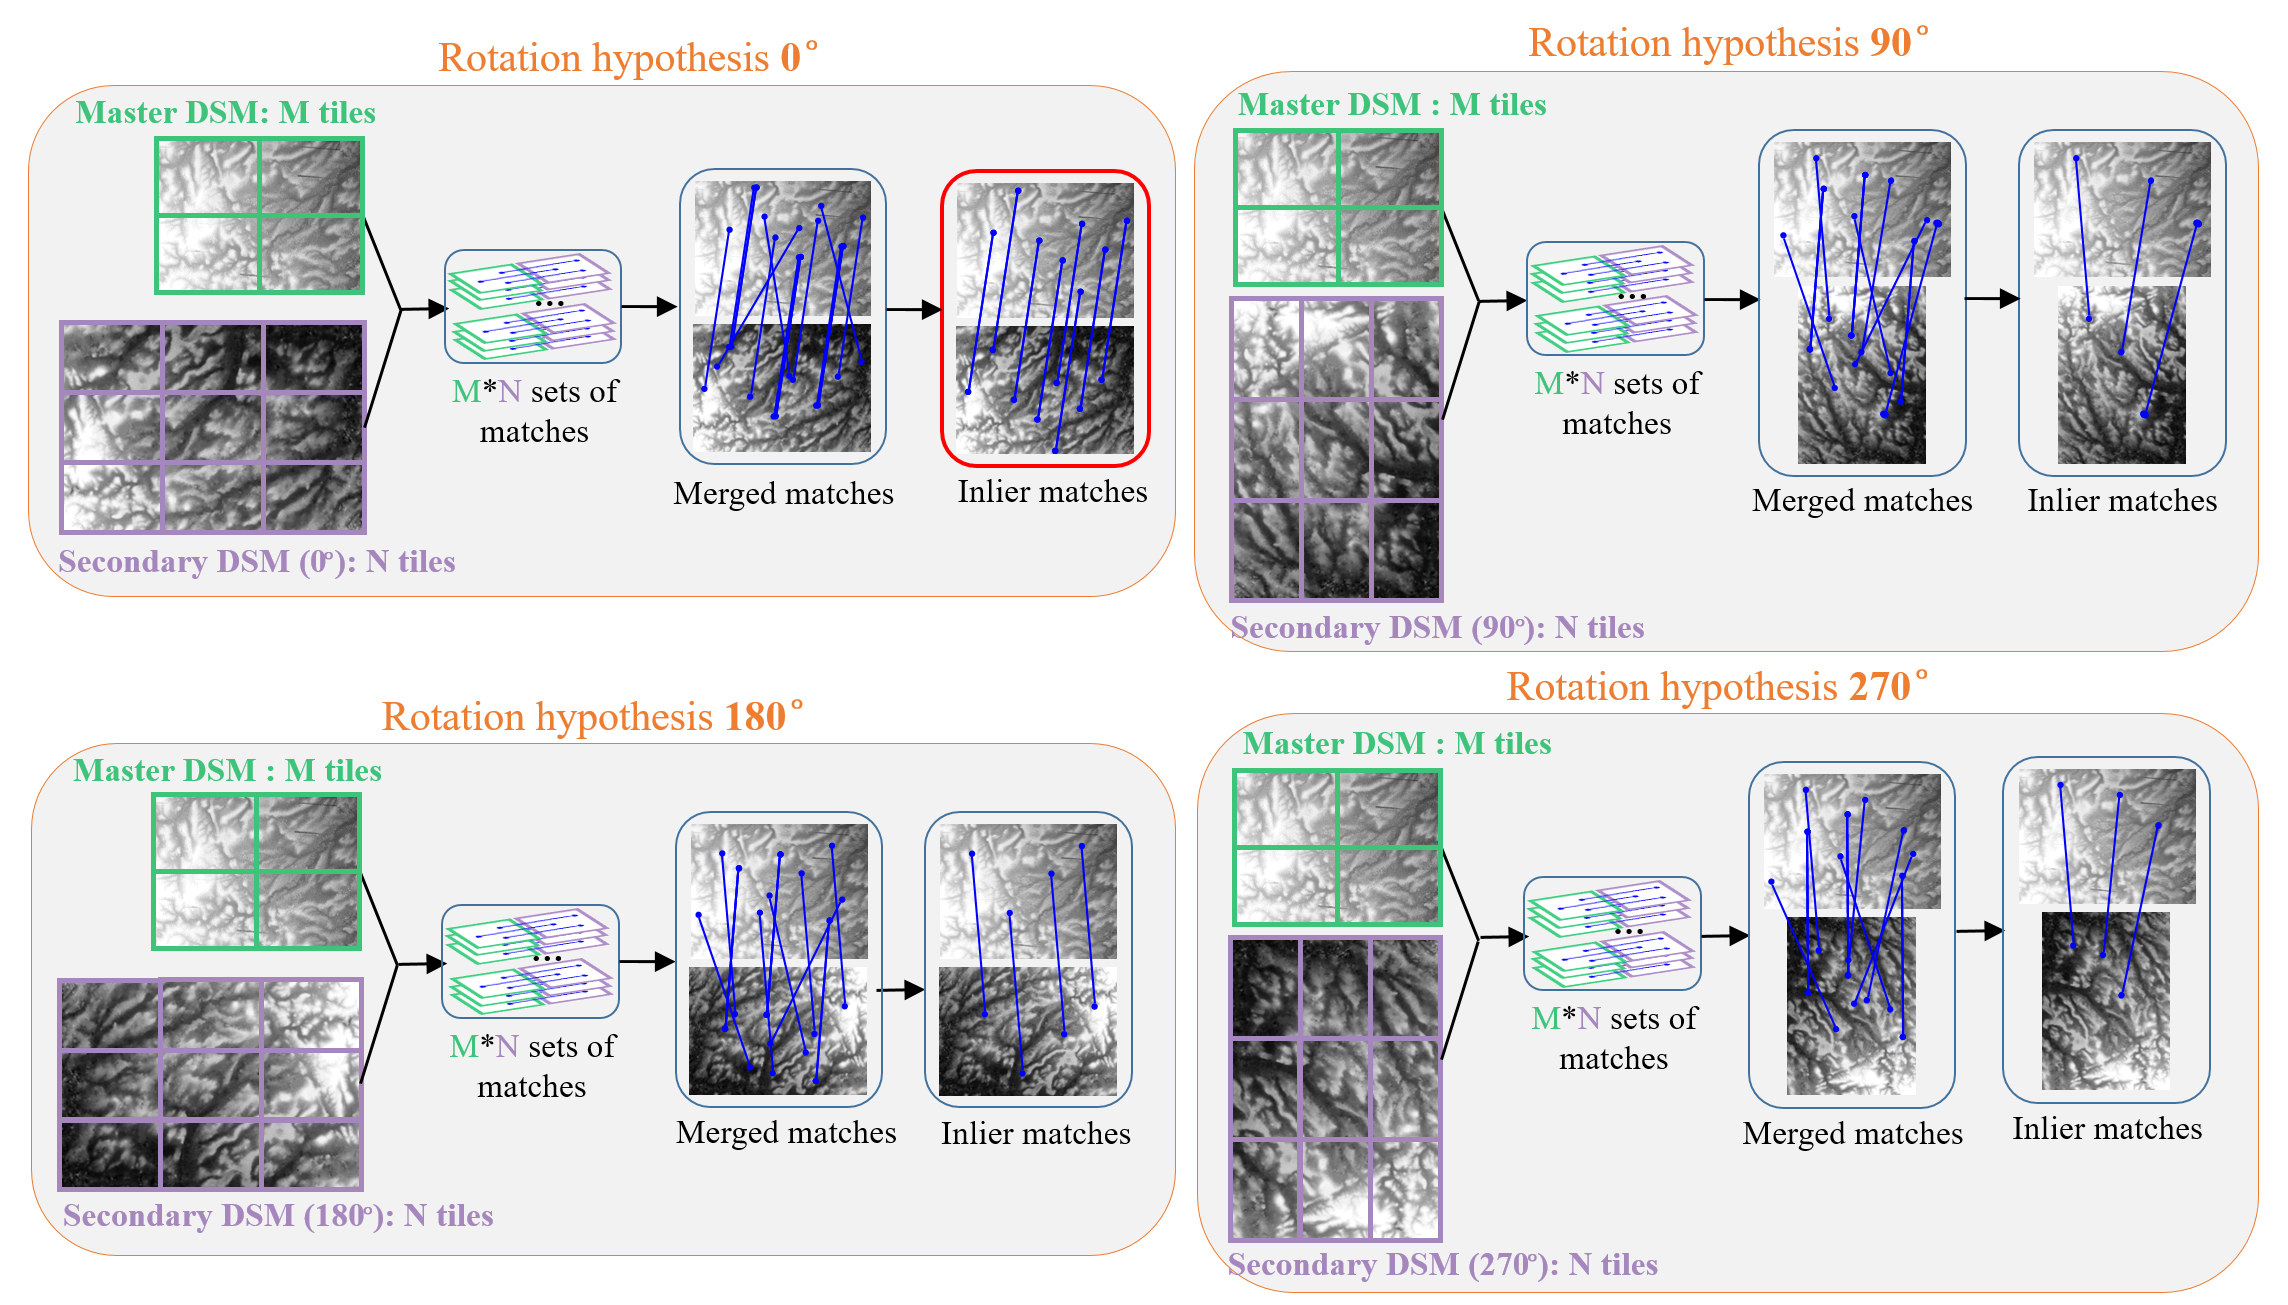
\includegraphics[width=1\columnwidth]{images/Chapitre3/dsm-RotHyp.png}
            \end{minipage}%
        }
        \caption{Rough co-registration by matching DSMs. (a) Workflow. DSMs are matched (with 4 rotation hypotheses combined with tiling scheme which are explained in (b), if the matching method is not rotation invariant), followed by projecting the inlier matches onto ground to build 3D Helmert transformation model. (b) Four rotation hypotheses combined with tiling scheme. We rotate the secondary DSM by 90 $^\circ$ four times to match with master DSM and keep the best one with the largest number of RANSAC inliers (red rectangle). Tiling scheme is applied during each hypothesis, with both DSMs croped into tiles followed by matching all the tile pairs and merging the matches.}
        \label{WorkflowDSM}
    \end{center}
\end{figure*}

%\begin{figure*}[htbp]
%    \begin{center}
%        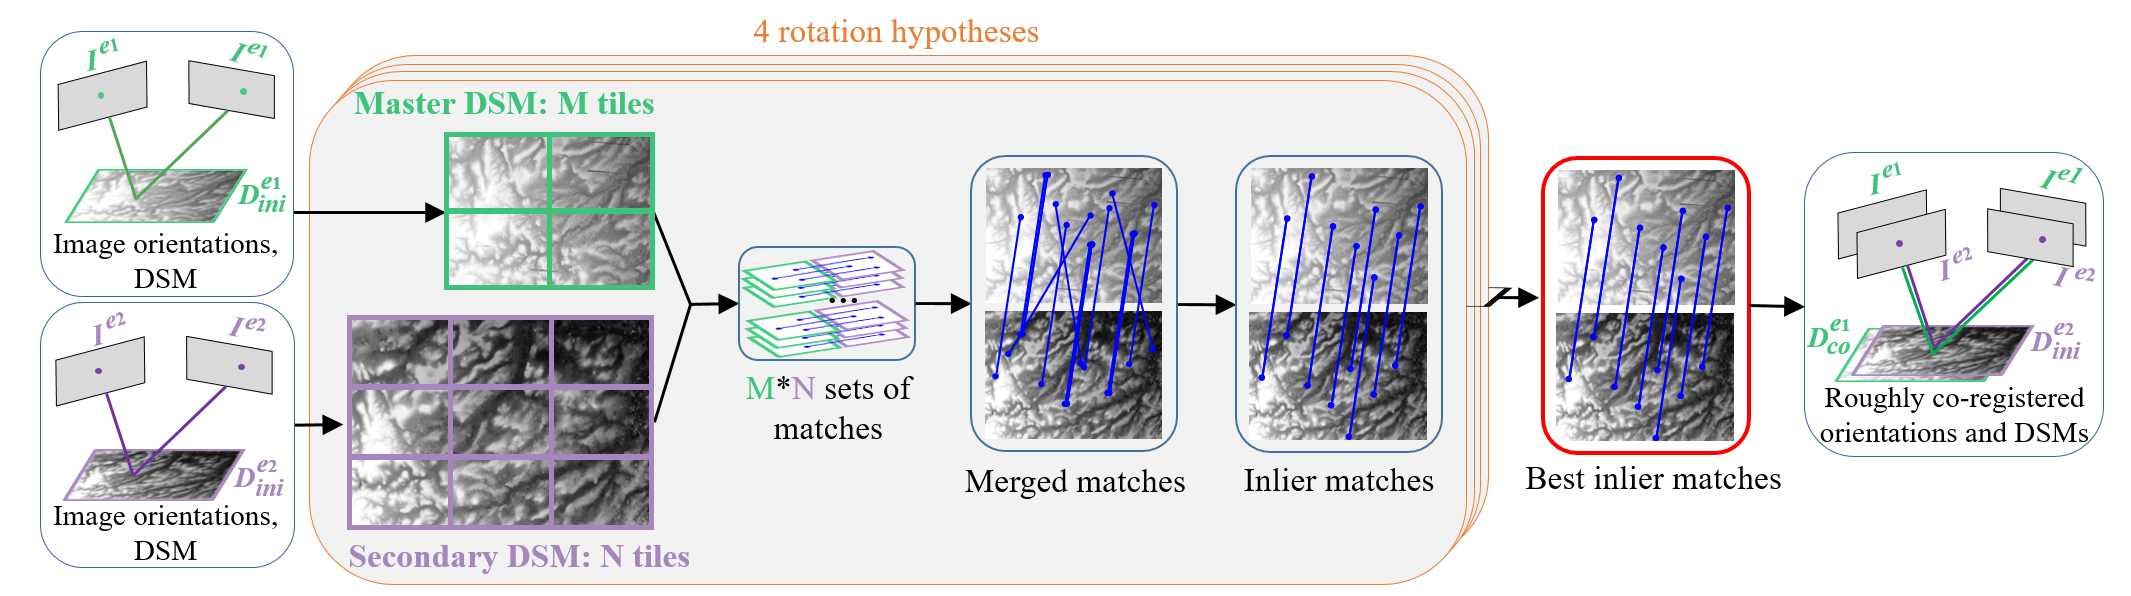
\includegraphics[width=1\columnwidth]{images/Chapitre3/dsm.png}
%        \caption{Rough co-registration by matching DSMs.}
%        \label{Flow-process diagram}
%    \end{center}
%\end{figure*}
%
%\begin{figure*}[htbp]
%    \begin{center}
%        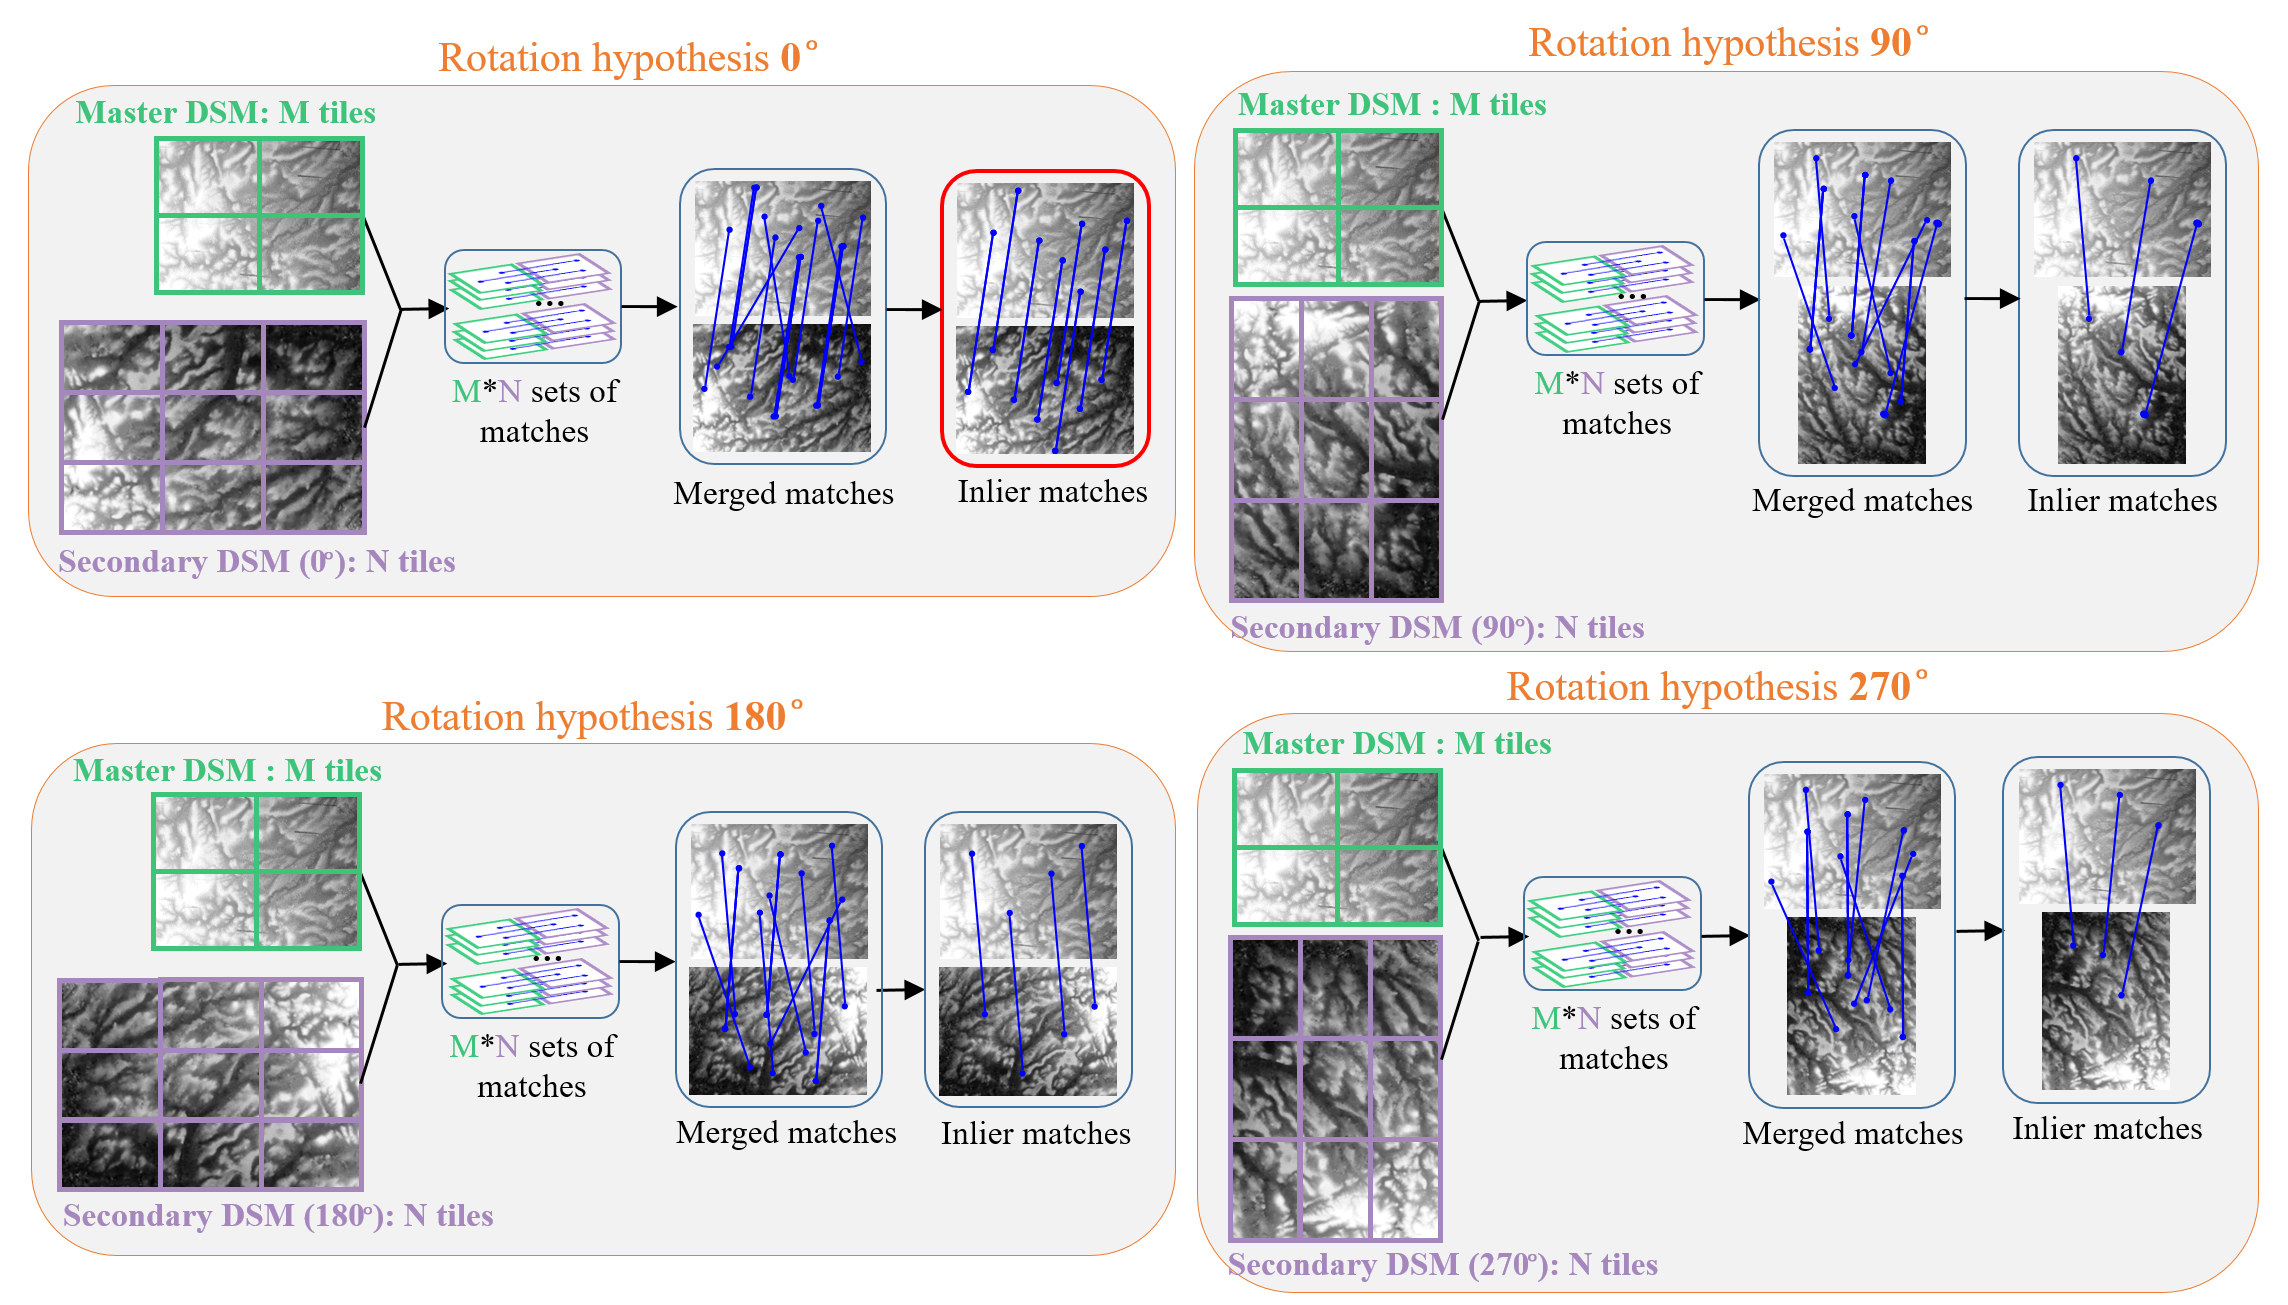
\includegraphics[width=0.8\columnwidth]{images/Chapitre3/dsm-RotHyp.png}
%        \caption{4 rotation hypotheses of matching DSMs.}
%        \label{Flow-process diagram}
%    \end{center}
%\end{figure*}

The DSM is converted to grayscale image as follows:\\
\begin{enumerate}
    \item Calculate the standard deviation of the DSM elevation;
    \item Pixels with elevations larger than double the standard deviation are considered outliers and therefore ignored;
    \item Transform the inlier pixels to the range of [0-255], resulting in grayscale image.
    \item Apply wallis filter on the grayscale image to get rid of uneven illumination, resulting in more informative image.
\end{enumerate}
\par
Matching DSMs/orthophotos has the following merits:
\begin{enumerate}
    \item Redundancy caused by the forward and side overlapping areas is removed;
    \item It implicitly enables a follow-up search for globally consistent inliers;
    \item It decreases the combinatorial complexity caused by rotation ambiguity of P$\times$Q images;
    \item When matching DSMs, robust matches can be expected even under extreme scene changes, as 3D landscape generally provide stable information over time.
\end{enumerate}

DSMs/orthophotos are usually large images as they have larger extent than original images.
Learned matching methods like SuperGlue often underperform on large images as they are either trained on small images to run real-time or with limited spatial resolution of CNN feature maps. We propose a \textit{one-to-many tiling scheme} to make up for the deficiency. 
\par
The \textit{one-to-many tiling scheme} is performed as follows (Figure~\ref{WorkflowImgPair}(a)):\\
\begin{enumerate}
    \item Crop both the master and secondary images into M and N tiles of certain size, respectively;
    \item Apply matching on M$\times$N tile pairs individually;
    \item Merge the matches and perform RANSAC based on 2D similarity transformation to remove outliers.
\end{enumerate}

The \textit{one-to-many tiling scheme} can be combined with \textit{4 rotation hypotheses} when the matching method is both unsatisfactory on large images and not rotation invariant, as shown in Figure~\ref{WorkflowImgPair}(b).
Both \textit{one-to-many tiling scheme} and \textit{4 rotation hypotheses} would not be applied when matching method that is both satisfactory on large images and rotation invariant (e.g. SIFT) is adopted.
\par
The matching DSMs/orthophotos strategy works as follows:\\
\begin{enumerate}
    \item Transform DSMs to grayscale images if the DSMs are to be matched.
    \item Match DSMs/orthophotos (with or without \textit{one-to-many tiling scheme} and \textit{4 rotation hypotheses}, depending on whether the matching method is satisfactory on large images and rotation invariant), giving rise to one set of matches $M({\mathbf{K}^{e_1},\mathbf{K}^{e_2}})$ ($\mathbf{K}^{e_i}$ represents keypoints in DSM $D^{e_i}$ or orthophoto $Op^{e_i}$).
    %\item Run RANSAC on matches based on 2D similarity transformation model to remove outliers.
    \item Sample matches $M({\mathbf{K}^{e_1},\mathbf{K}^{e_2}})$ iteratively to compute the 2D similarity transformation RANSAC model:
\begin{equation}
\left [ \begin{array}{c}
{K}_x^{e_2}\\
{K}_y^{e_2}
\end{array}
\right ] =\lambda \cdot { \left[ \begin{array}{cc}
    cos\theta & sin\theta\\
    -sin\theta & cos\theta
    \end{array} 
    \right ]} \cdot {\left [ \begin{array}{c}
    {K}_x^{e_1}\\
    {K}_y^{e_1}
    \end{array}
    \right ]} + \left [ \begin{array}{c}
\Delta_x\\
\Delta_y
\end{array}
\right ]. \label{eq:2DSim}
\end{equation}

%   \begin{equation*}
%       {KG_i^{e_2}} = \lambda \cdot \mathbf{R} \cdot {KG_i^{e_1}} + \mathbf{T} , \quad i \in [1,3] \label{eq:3Dsim}
%   \end{equation*}
    where $\lambda$ is the scale factor, $\theta$ is the in-plane rotation angle and $\left [ \begin{array}{c}
    \Delta_x, \Delta_y
    \end{array}
    \right ]$ $^{^T}$ is the translation vector.
    %$\mathbf{T}$ is the translation vector and $\mathbf{R}$ is the rotation matrix.
    We set the number of RANSAC iterations to 1000, and consider matches within $T_r$ of its predicted position as inliers. In our experiment, {$T_r$ was set to 15 pixels.}
    \item Project the inlier matches onto ground to calculate 3D Helmert transformation parameters.
\end{enumerate}




%\subsubsection{SIFT}
%\subsubsection{SuperGlue}

\section{Experiments}
As described in the previous section, we provide 3 pipelines out of 2 strategies to perform rough co-registration:\\
\begin{enumerate}
    \item Match image pairs: hereinafter referred to as \textit{ImgPairs};
    \item Match orthophotos: hereinafter referred to as \textit{Ortho};
    \item Match DSMs: hereinafter referred to as \textit{DSM}.
\end{enumerate}
For each pipeline, we employ either SIFT or SuperGlue as the feature matching method, giving rise to 6 methods:\\
\begin{enumerate}
    \item $SIFT_{ImgPairs}$;
    \item $SuperGlue_{ImgPairs}$;
    \item $SIFT_{Ortho}$;
    \item $SuperGlue_{Ortho}$;
    \item $SIFT_{DSM}$;
    \item $SuperGlue_{DSM}$;
\end{enumerate}
In the following we introduce the datasets and the evaluation criteria, as well as comparison of the 6 methods.\\
For each dataset, one epoch would be chosen as the reference epoch, the remaining epochs would be treated as free epochs. The rough co-registration is applied on each free epoch and the reference epoch to obtain the co-registered image orientations in the frame of the reference epoch.\\

\subsection{Datasets}
%Frejus, Pezenas, Kobe\\
We tested our method on three datasets: Pezenas, Fr{\'e}jus and Kobe. Details of the datasets are listed in Table~\ref{Data details} and Figure~\ref{FrejusData},~\ref{PezenasData}, ~\ref{KobeData}.
\par
\paragraph{Fr{\'e}jus} It is a 15 $km^2$ rectangular area located in Fr{\'e}jus, a commune in southeastern France. The area is mainly covered with buildings along with scattered farmlands, except a half-moon-shaped bay located in south. We have four sets of images acquired in 1954, 1966, 1970 and 2014. The epoch 2014 was acquired with the IGN's digital metric camera ~\cite{souchon2010ign}, and is treated as the ground truth (GT) during our processing (in other words, the epoch 2015 is chosen as the reference epoch (\textcolor{red}{explain reference epoch beforehand})). The area exhibits drastic scene changes in the 60-year period, as can be seen in Figure~\ref{FrejusData}.\\
\paragraph{Pezenas} It is a 420 $km^2$ rectangular area located in Pezenas in the Occitanie region in southern France. The area is mainly covered with vegetation and several sparsely populated urban zones. We have at our disposal three sets of images acquired in 1971, 1981 and 2015. The epoch 2015 is treated as GT. The area exhibits changes in scene appearance in the 44-year period.\\
\paragraph{Kobe} It is a 90 $km^2$ area of irregular shape located in the north of Awaji Island, Japan. The well-known Kobe earthquake happened here in January 1995. We have two sets of images: pre-event acquired in 1991 and post-event acquired in 1995. It is mainly covered with mountain area and narrow urban zones along the sea. There is no GT, therefore the recent epoch (i.e. epoch 1995) is treated as reference epoch. In this dataset we are interested in localizing the earthquake fault.
\begin{table}[htbp]
    \scriptsize %\footnotesize
    \centering
    \begin{tabular}{||l|c|c|c|c||c|c|c|c||c|c||}\hline
        &\multicolumn{4}{c||}{Fr{\'e}jus}&\multicolumn{4}{c||}{Pezenas}&\multicolumn{2}{c||}{Kobe}\\\hline
                &E1954&E1966&E1970&E2014&E1971&E1981&\multicolumn{2}{c||}{E2015}&E1991&E1995\\\hline\hline
        F [pix]&23350&10230&10230&\color{black}18281&7589&7607&9967.5&9204.5&7662&7662\\
        %Size [mm]&\color{black}300,300&\color{black}180,180&\color{black}180,180&99.28,72.42&230230&230230&47,35&50,36&212212&212,212\\
        Wid [mm]&300&180&180&99.28&230&230&47&50&212&212\\
        Hei [mm]&300&180&180&72.42&230&230&35&36&212&212\\
        GSD [m]&\color{black}0.11&\color{black}0.17&0.17&0.35&0.32&0.59&0.46&0.5&0.5&0.18\\
        F. o.&60\%&60\%&60\%&60\%&   60\%&60\%&60\%&60\%&   65\%&65\%\\
        S. o.&20\%&30\%&30\%&30\%&   20\%&20\%&50\%&50\%&   35\%&65\%\\
        H  [m]&2500&1700&1700&6500&2400&4500&4600&4600&3800&1400\\
        Nb &19&15&19&33&57&27&308&74&15&83\\\hline
        
        
%       &E1971&E1981&\multicolumn{2}{c||}{E2015}&E1954&E1966&E1970&E2014&E1991&E1995\\\hline\hline
%       F [pix]&7589&7607&9967.5&9204.5&23350&10230&10230&\color{black}18281&7662&7662\\
%       %Size [mm]&230230&230230&47,35&50,36&\color{black}300,300&\color{black}180,180&\color{black}180,180&99.28,72.42&212212&212,212\\
%       Wid [mm]&230&230&47&50&300&180&180&99.28&212&212\\
%       Hei [mm]&230&230&35&36&300&180&180&72.42&212&212\\
%       GSD [m]&0.32&0.59&0.46&0.5&\color{black}0.11&\color{black}0.17&0.17&0.35&0.5&0.18\\
%       F. o.&   60\%&60\%&60\%&60\%&60\%&60\%&60\%&60\%&   65\%&65\%\\
%       S. o.&   20\%&20\%&50\%&50\%&20\%&30\%&30\%&30\%&   35\%&65\%\\
%       H  [m]&2400&4500&4600&4600&2500&1700&1700&6500&3800&1400\\
%       Nb &57&27&308&74&19&15&19&33&15&83\\\hline
    \end{tabular}
    \caption{Dataset details of Fr{\'e}jus, Pezenas and Kobe. The 2015 acquisition of Pezenas is obtained with two sets of camera. E stands for epoch, F means focal length, Wid and Hei are the width and height of image, GSD is the ground sampling distance, F.o. and S.o. are forward and side overlap, H is the flying height, Nb is the number of images.}
    \label{Data details}
\end{table}


\begin{figure*}[htbp]
    \begin{center}
        \subfigure[Fr{\'e}jus 1954]{
            \begin{minipage}[t]{0.38\linewidth}
                \centering
                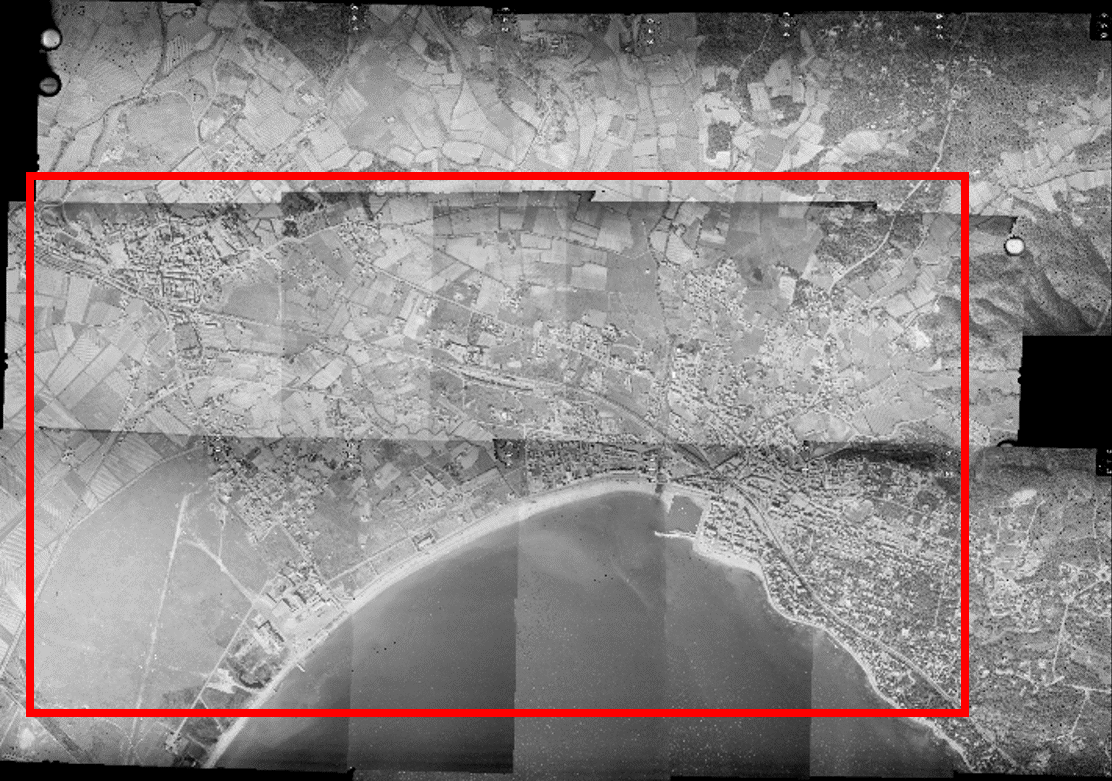
\includegraphics[width=5.45cm]{images/Chapitre3/Frejus1954.png}
            \end{minipage}%
        }
        \subfigure[Fr{\'e}jus 1966]{
            \begin{minipage}[t]{0.58\linewidth}
                \centering
                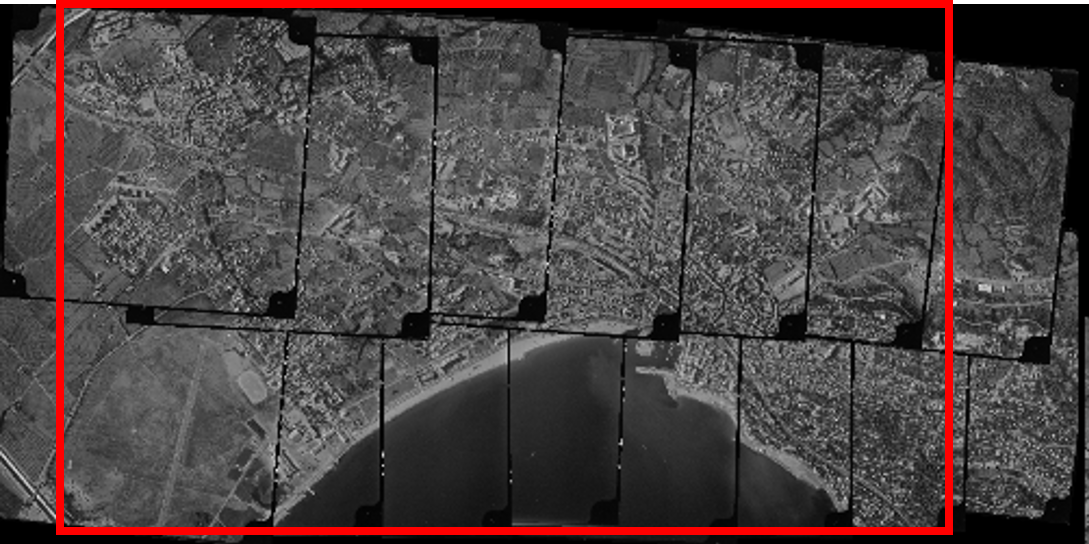
\includegraphics[width=7.8cm]{images/Chapitre3/Frejus1966.png}
            \end{minipage}%
        }
        \subfigure[Fr{\'e}jus 1970]{
    \begin{minipage}[t]{0.48\linewidth}
        \centering
        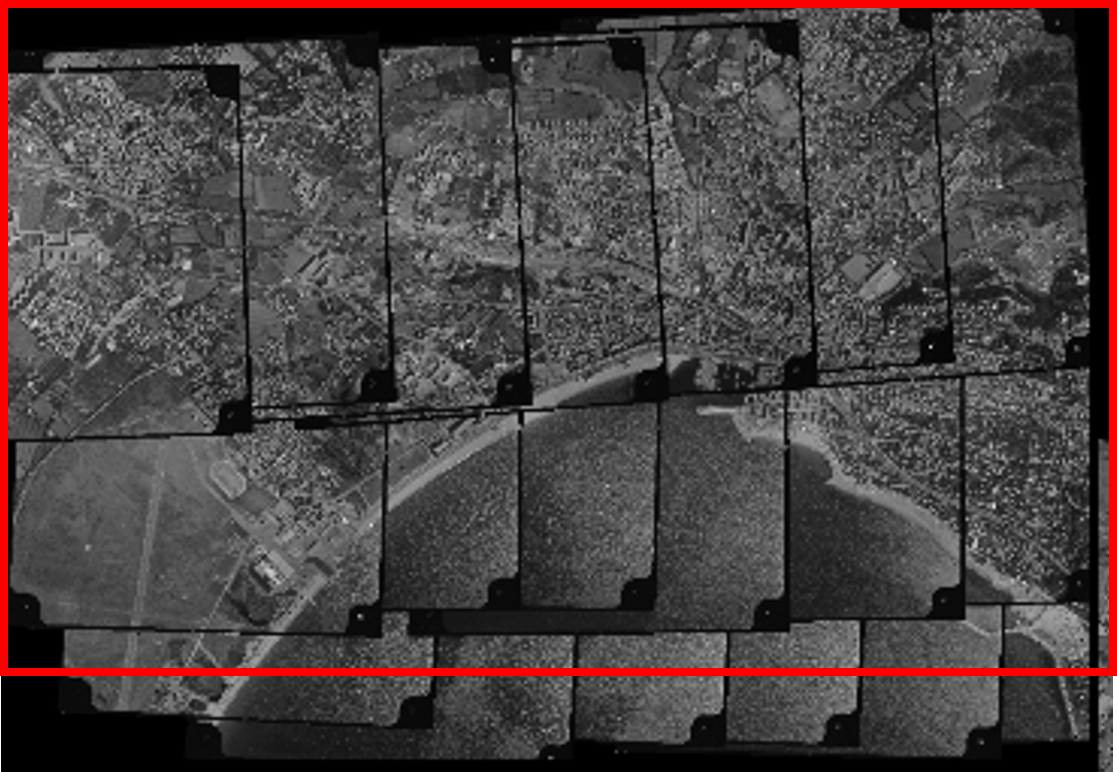
\includegraphics[width=6.8cm]{images/Chapitre3/Frejus1970.png}
    \end{minipage}%
}
\subfigure[Fr{\'e}jus 2014]{
    \begin{minipage}[t]{0.48\linewidth}
        \centering
        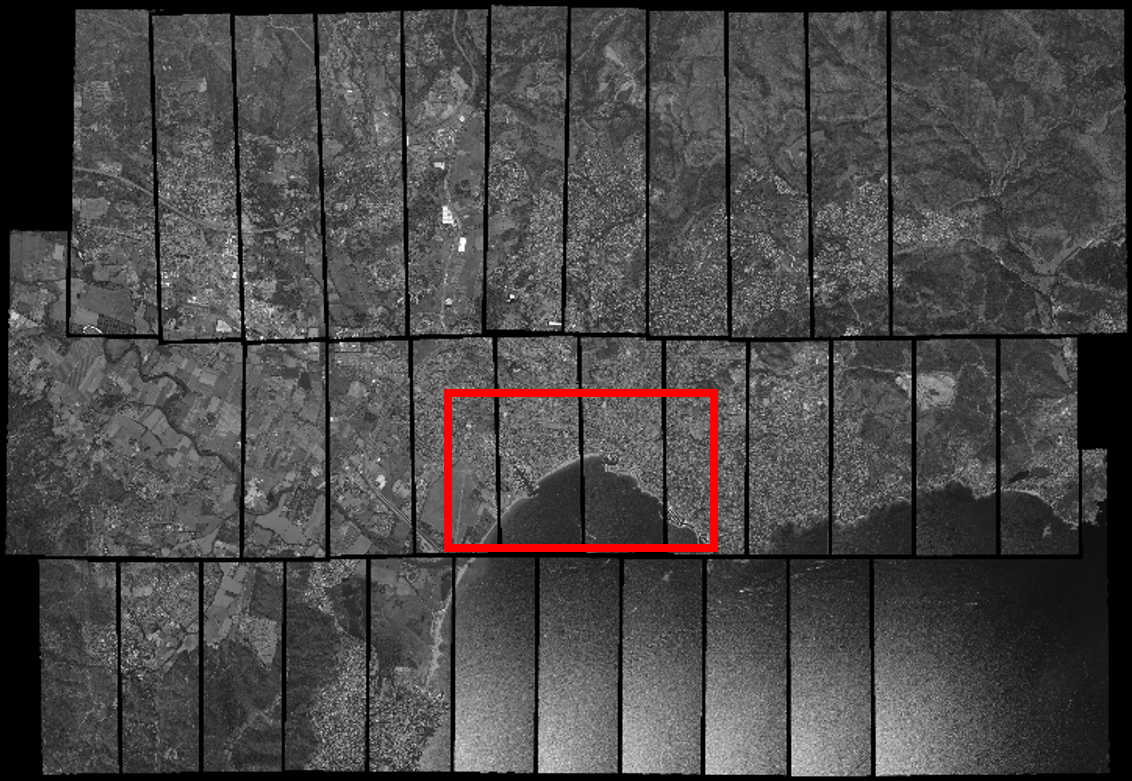
\includegraphics[width=6.6cm]{images/Chapitre3/Frejus2014.png}
    \end{minipage}%
}
        \caption{Images demonstration of different epochs in Fr{\'e}jus. The common zone of all the epochs is indicated by the red rectangles.}
        \label{FrejusData}
    \end{center}
\end{figure*} 


\begin{figure*}[htbp]
    \begin{center}
        \subfigure[Pezenas 1971]{
            \begin{minipage}[t]{0.31\linewidth}
                \centering
                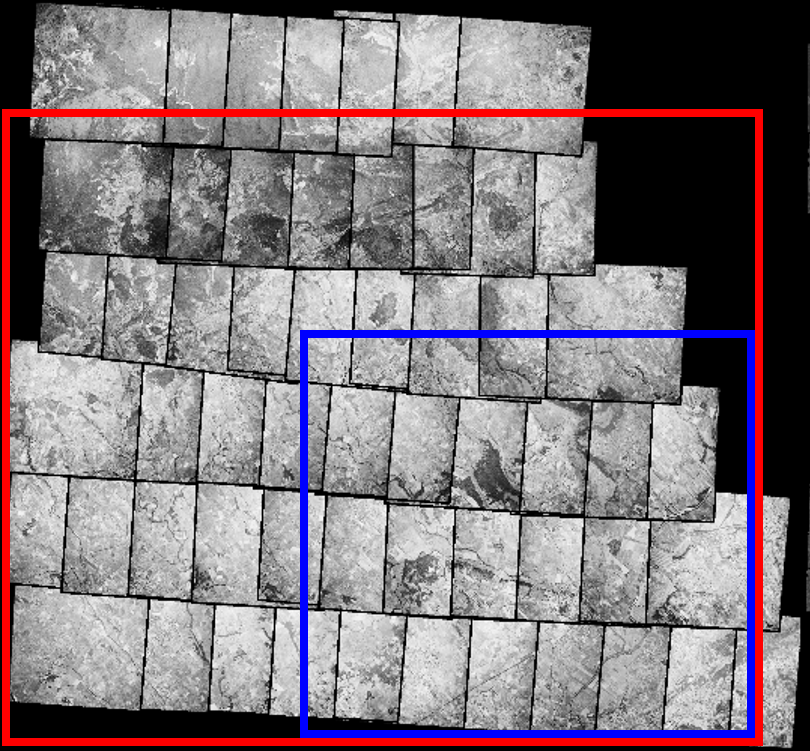
\includegraphics[width=4.4cm]{images/Chapitre3/Pezenas1971.png}
            \end{minipage}%
        }
        \subfigure[Pezenas 1981]{
            \begin{minipage}[t]{0.31\linewidth}
                \centering
                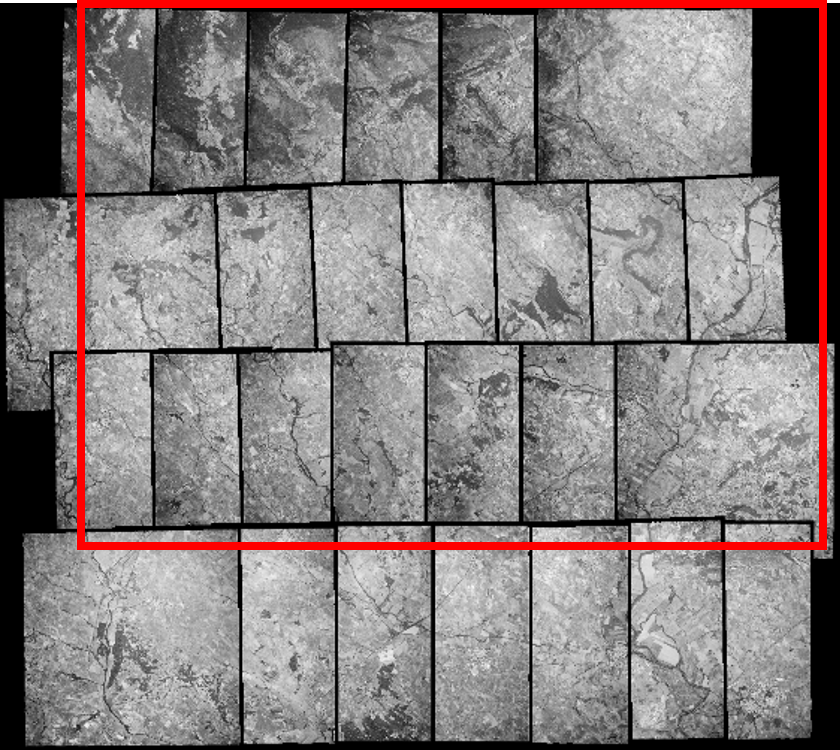
\includegraphics[width=4.5cm]{images/Chapitre3/Pezenas1981.png}
            \end{minipage}%
        }
        \subfigure[Pezenas 2015]{
            \begin{minipage}[t]{0.29\linewidth}
                \centering
                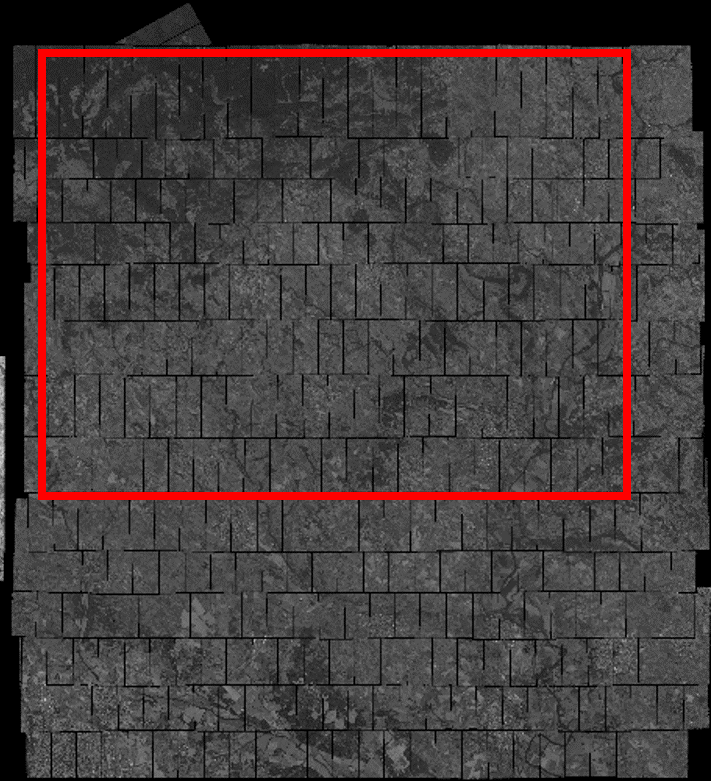
\includegraphics[width=3.9cm]{images/Chapitre3/Pezenas2015.png}
            \end{minipage}%
        }
        \caption{Images demonstration of different epochs in Pezenas. The common zone of all the epochs is indicated by the red rectangles.}
        \label{PezenasData}
    \end{center}
\end{figure*} 


\begin{figure*}[htbp]
    \begin{center}
        \subfigure[Kobe 1991]{
            \begin{minipage}[t]{1\linewidth}
                \centering
                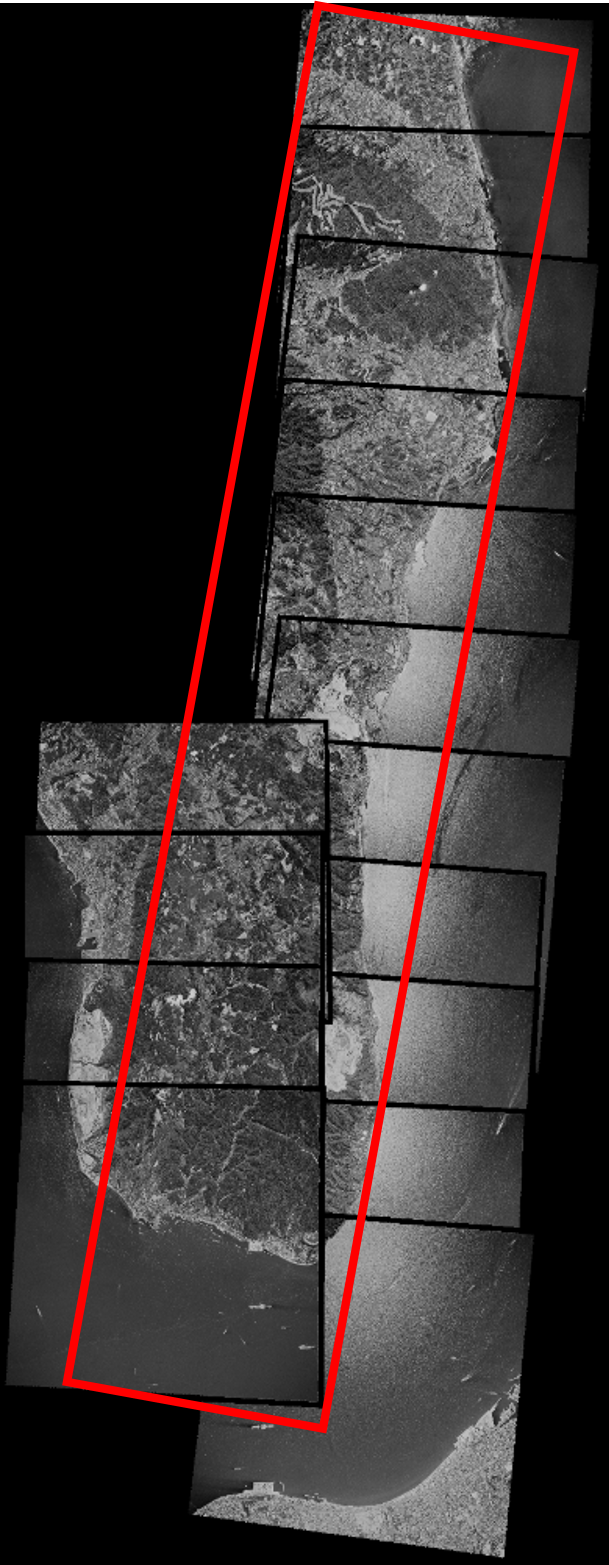
\includegraphics[height=13cm,angle=90]{images/Chapitre3/Kobe1991.png}
            \end{minipage}%
        }
        \subfigure[Kobe 1995]{
            \begin{minipage}[t]{1\linewidth}
                \centering
                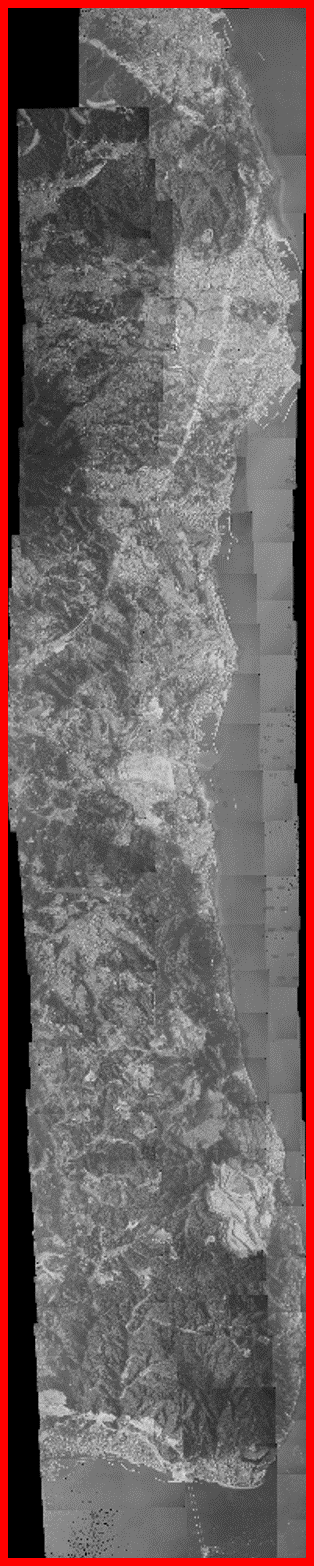
\includegraphics[height=13cm,angle=90]{images/Chapitre3/Kobe1995.png}
            \end{minipage}%
        }
        \caption{Images demonstration of different epochs in Kobe. The common zone of all the epochs is indicated by the red rectangles.}
        \label{KobeData}
    \end{center}
\end{figure*} 

%Show piled image of each epoch?
\subsection{Evaluation}
%\subsubsection{Qualitative evaluation}
%\subsubsection{Quantitative evaluation}
%(1)Matches visualization\\
%%inlier ratio (RANSAC and GT)\\
%(2)Ground check points\\
%(3)DoD\\
For each dataset, we manually measured 3 GCPs well distributed in the block. The application of 3 GCPs is twofold:\\
\begin{itemize}
    \item Based on the GCPs, a 3D Helmert transformation model between each free epoch and the reference epoch is built to obtain the GT co-registered orientations.
    \item GCPs are also treated as ground check points to evaluate the co-registered orientations calculated by our methods.
\end{itemize}
%as check points to evaluate the roughly co-registered orientations resulted by 6 methods:\\
In order to evaluate the results qualitatively and quantitatively, the following criterias would be applied:\\
\begin{itemize}
    \item Matches visualization: the match number of (1) total matches (i.e. matches before RANSAC), (2) GT inliers (matches located within $T_r$ of the position predicted by the GT co-registered orientations) and (3) RANSAC inliers (matches that survived RANSAC in our methods) would be calculated and displayed; in the meantime, the RANSAC inliers would be visualized and demonstrated.
    \item Ground check points: the co-registered orientations calculated by our methods would be used to triangulate the ground check points and the coordinate differences \textcolor{red}{(explain the diff means the mean diff of x, y and z)} will be displayed. The better the epochs co-register, the smaller the difference is.
    \item DoD: the co-registered orientations calculated by our methods would be used to calculate DSMs in order to generate DoD. Ideally the DoD should only display the scene changes. If the dome effect appears, it indicates the systematic errors caused by poorly estimated camera parameters.   
\end{itemize}

\subsection{Comparison}
%分三部分分别展示3组数据的结果
%3*2 methods:
%1张表表示6种方法的(1)和(2),1张大图放6种方法的DoD, inlier tie pt图(R3D, DSM, ortho各3张(无点图,SIFT点图,SpG点图))

\subsubsection{Matches visualization}

\begin{figure*}[htbp]
    \begin{center}
        \subfigure[Image pairs]{
            \begin{minipage}[t]{0.65\linewidth}
                \centering
                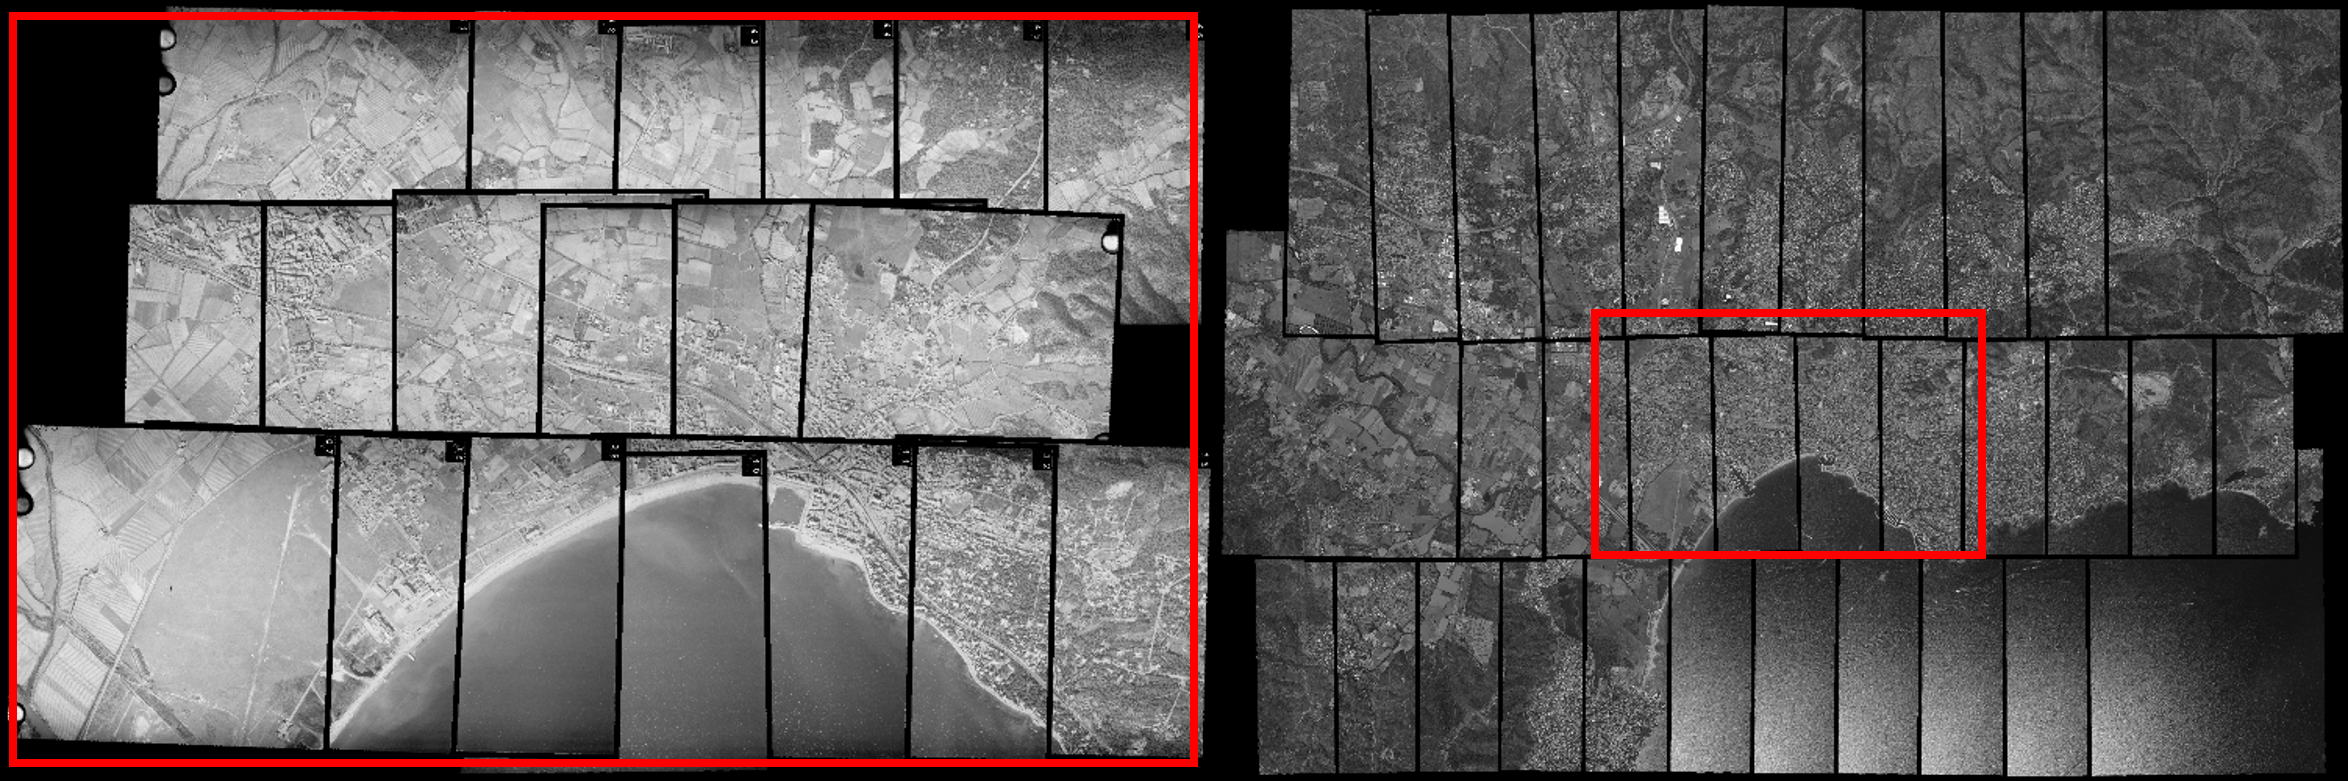
\includegraphics[width=8.8cm]{images/Chapitre3/Pseudo-Ortho-MEC-Malt_Tapas_1954_Ortho-MEC-Malt_2014.png}
            \end{minipage}%
        }
        \subfigure[Match number (\textit{ImgPairs})]{
    \begin{minipage}[t]{0.3\linewidth}
        \centering
        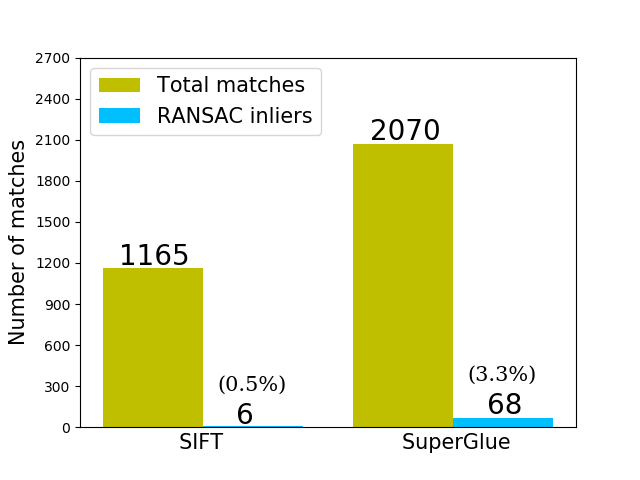
\includegraphics[width=4.8cm]{images/Chapitre3/PlotCurves_Pseudo-Ortho-MEC-Malt_Tapas_1954_Ortho-MEC-Malt_2014.png}
    \end{minipage}%
}
        \subfigure[$SIFT_{ImgPairs}^{RANSAC Inliers}$]{
            \begin{minipage}[t]{0.48\linewidth}
                \centering
                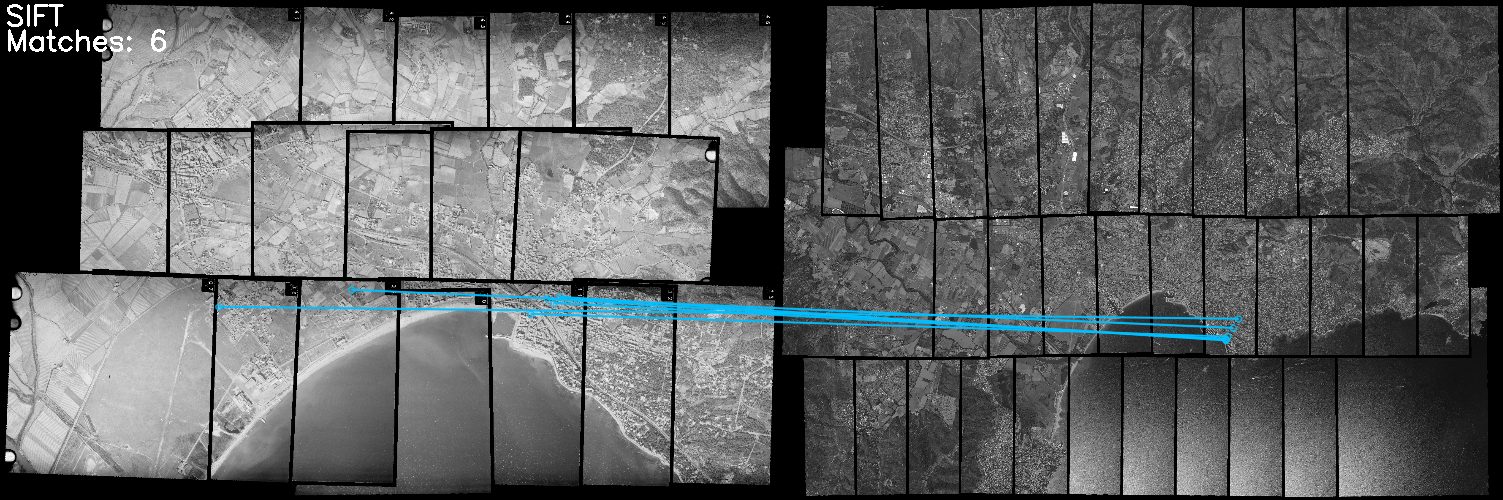
\includegraphics[width=6.8cm]{images/Chapitre3/Pseudo-Homol-SIFT2Step_1954-2014-Rough-2DRANSAC-GlobalR3D-PileImg_Ortho-MEC-Malt_Tapas_1954_Ortho-MEC-Malt_2014.png}
            \end{minipage}%
        }
        \subfigure[$SuperGlue_{ImgPairs}^{RANSAC Inliers}$]{
            \begin{minipage}[t]{0.48\linewidth}
                \centering
                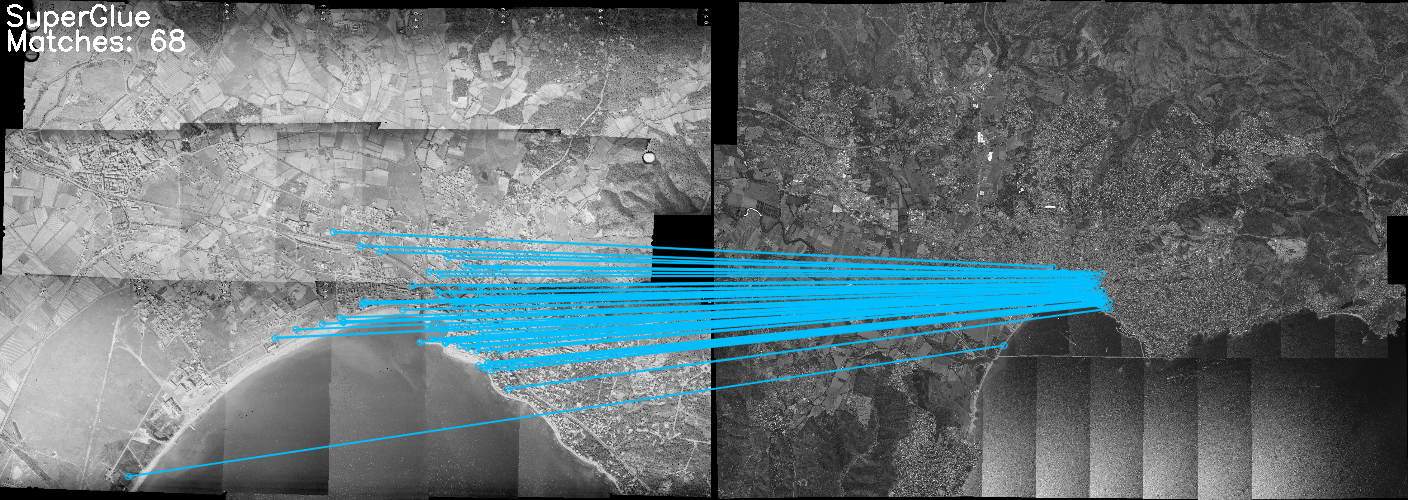
\includegraphics[width=6.8cm]{images/Chapitre3/Pseudo-Homol-SuperGlue_1954-2014-GlobalR3D-PileImg_Ortho-MEC-Malt_Tapas_1954_Ortho-MEC-Malt_2014.png}
            \end{minipage}%
        }
        \caption{Result of matching image pairs of Fr{\'e}jus 1954 and 2014. (a) Demonstration of image pairs to be matches. The images in the same epoch are projected onto ground}
        \label{Match result}
    \end{center}
\end{figure*} 



\begin{figure*}[htbp]
    \begin{center}
        \subfigure[Orthophotos]{
    \begin{minipage}[t]{0.65\linewidth}
        \centering
        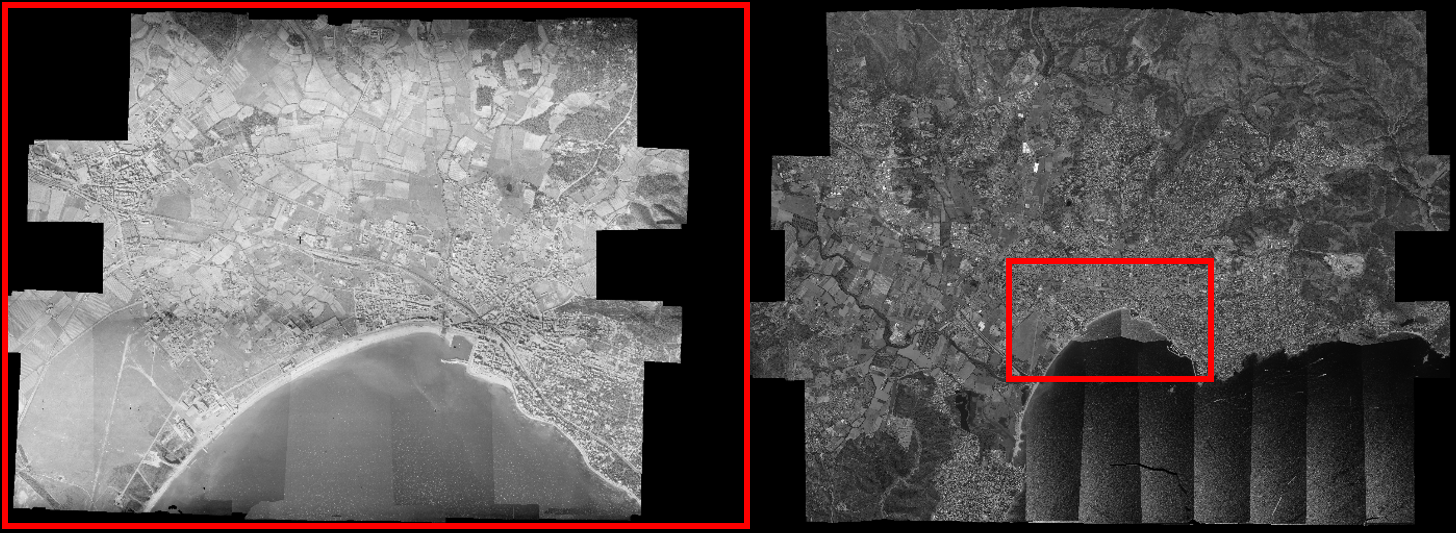
\includegraphics[width=8.8cm]{images/Chapitre3/Ortho-MEC-Malt_Tapas_1954_Ortho-MEC-Malt_2014.png}
    \end{minipage}%
}
\subfigure[Match number (\textit{Ortho})]{
    \begin{minipage}[t]{0.3\linewidth}
        \centering
        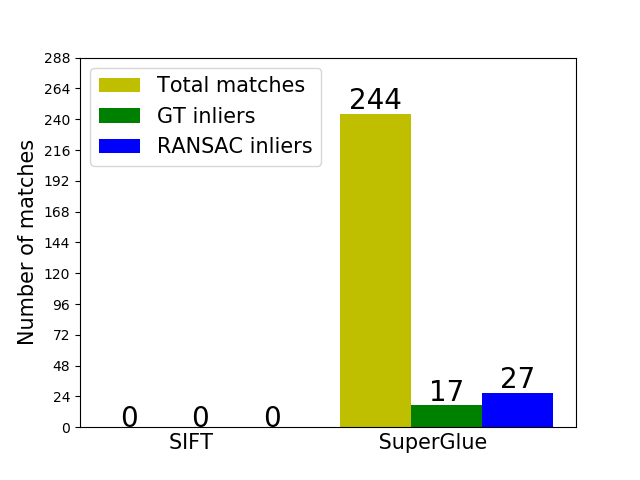
\includegraphics[width=4.8cm]{images/Chapitre3/PlotCurves_Ortho-MEC-Malt_Tapas_1954_Ortho-MEC-Malt_2014.png}
    \end{minipage}%
}
        \subfigure[$SIFT_{Ortho}^{RANSAC Inliers}$]{
            \begin{minipage}[t]{0.48\linewidth}
                \centering
                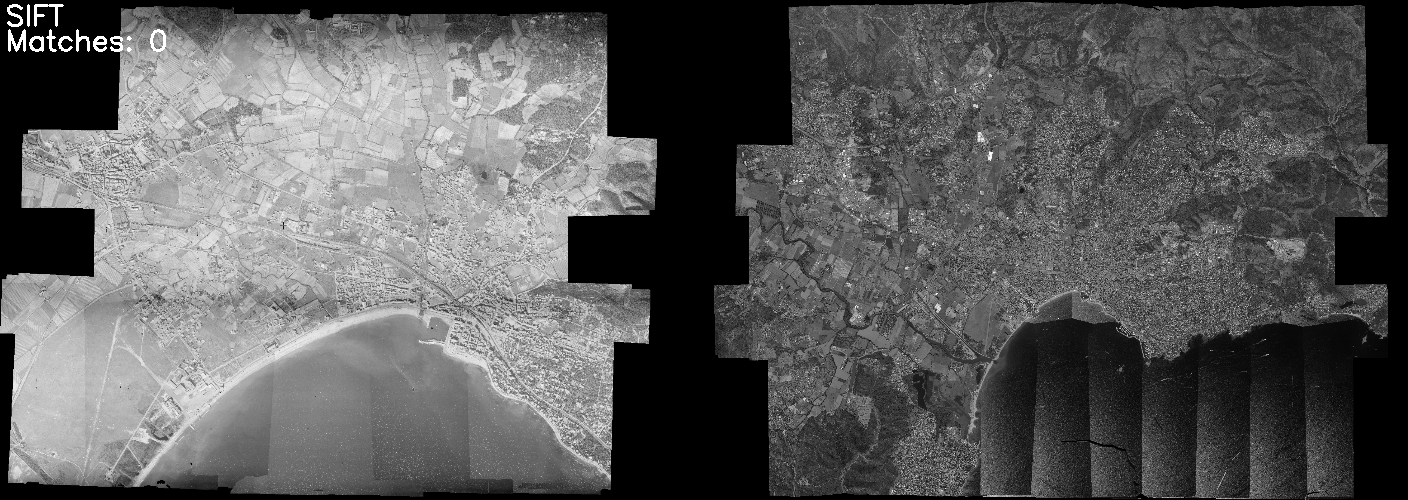
\includegraphics[width=6.8cm]{images/Chapitre3/Homol-SIFT-2DRANSAC_Ortho-MEC-Malt_Tapas_1954_Ortho-MEC-Malt_2014.png}
            \end{minipage}%
        }
        \subfigure[$SuperGlue_{Ortho}^{RANSAC Inliers}$]{
            \begin{minipage}[t]{0.48\linewidth}
                \centering
                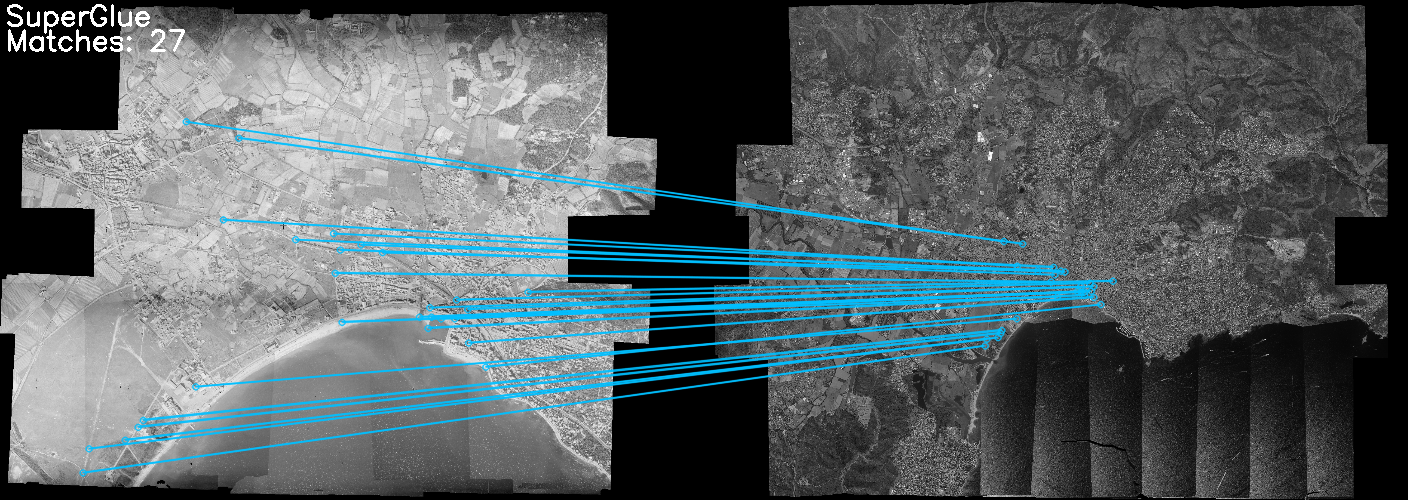
\includegraphics[width=6.8cm]{images/Chapitre3/Homol-SubPatch_R270-2DRANSAC_Ortho-MEC-Malt_Tapas_1954_Ortho-MEC-Malt_2014.png}
            \end{minipage}%
        }
        \caption{Result of matching orthophotos of Fr{\'e}jus 1954 and 2014.}
        \label{Match result}
    \end{center}
\end{figure*} 

\begin{figure*}[htbp]
    \begin{center}
        \subfigure[DSMs]{
    \begin{minipage}[t]{0.65\linewidth}
        \centering
        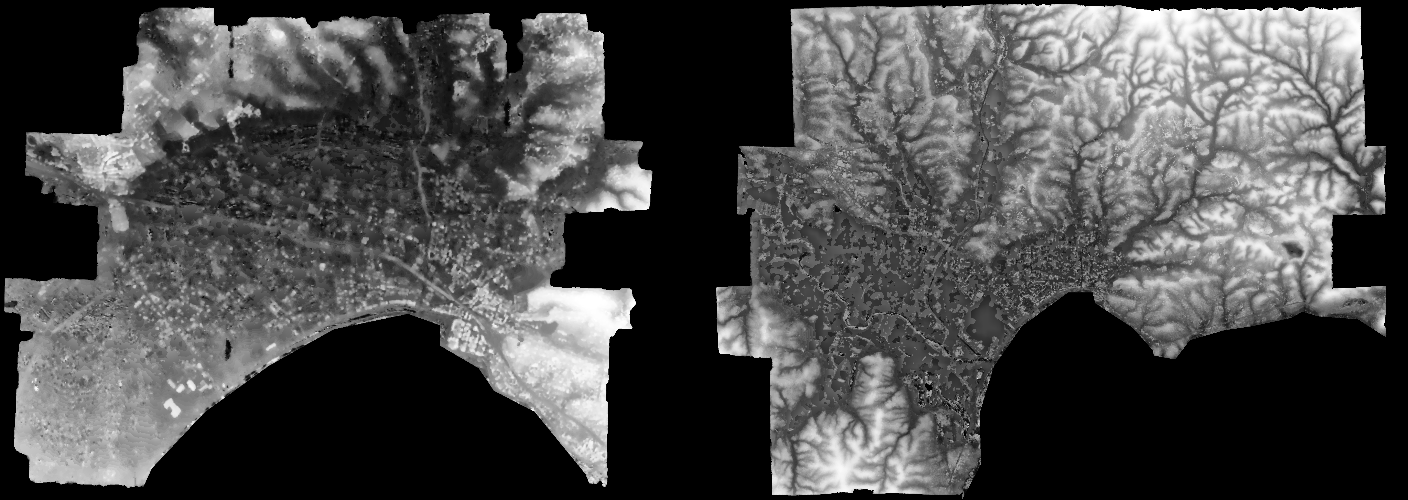
\includegraphics[width=8.8cm]{images/Chapitre3/MEC-Malt_Tapas_1954_MEC-Malt_2014.png}
    \end{minipage}%
}
\subfigure[Match number (\textit{DSM})]{
    \begin{minipage}[t]{0.3\linewidth}
        \centering
        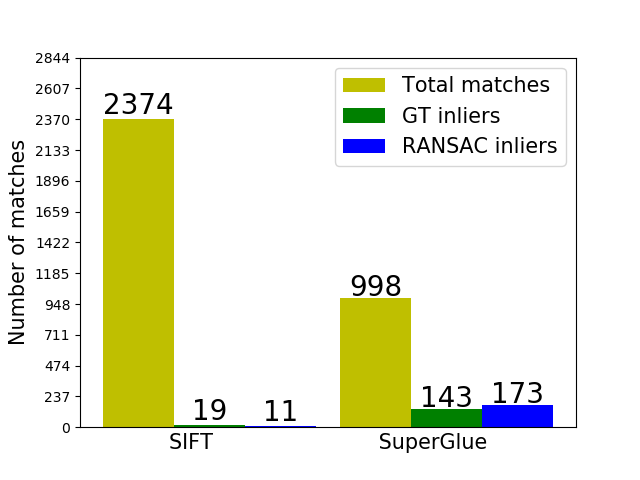
\includegraphics[width=4.8cm]{images/Chapitre3/PlotCurves_MEC-Malt_Tapas_1954_MEC-Malt_2014.png}
    \end{minipage}%
}
        \subfigure[$SIFT_{DSM}^{RANSAC Inliers}$]{
            \begin{minipage}[t]{0.48\linewidth}
                \centering
                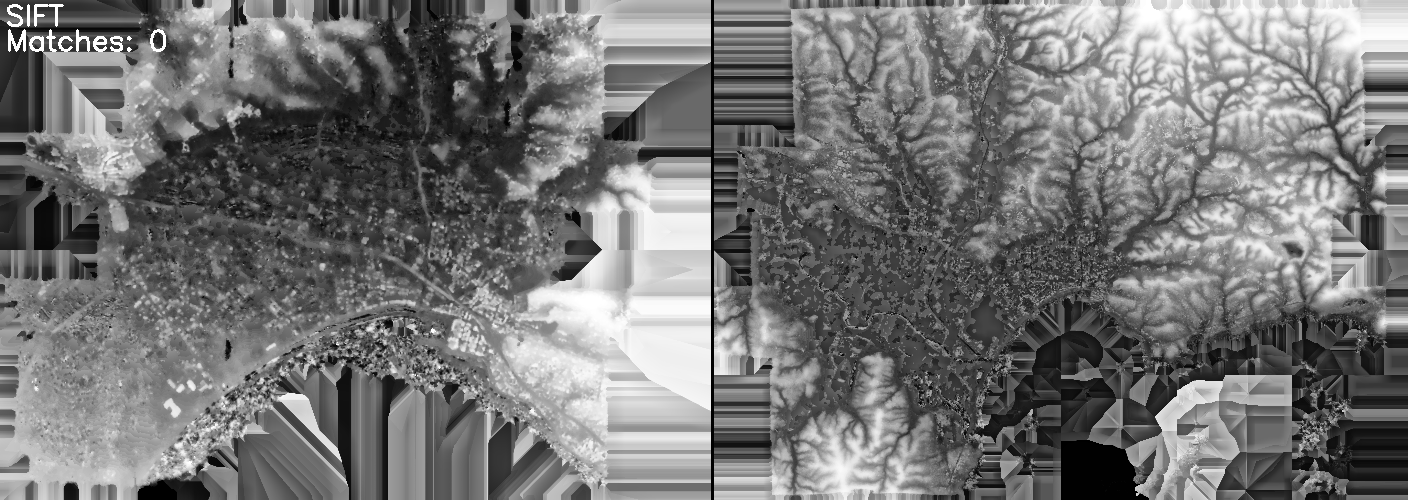
\includegraphics[width=6.8cm]{images/Chapitre3/Homol-SIFT-2DRANSAC_MEC-Malt_Tapas_1954_MEC-Malt_2014.png}
            \end{minipage}%
        }
        \subfigure[$SuperGlue_{DSM}^{RANSAC Inliers}$]{
            \begin{minipage}[t]{0.48\linewidth}
                \centering
                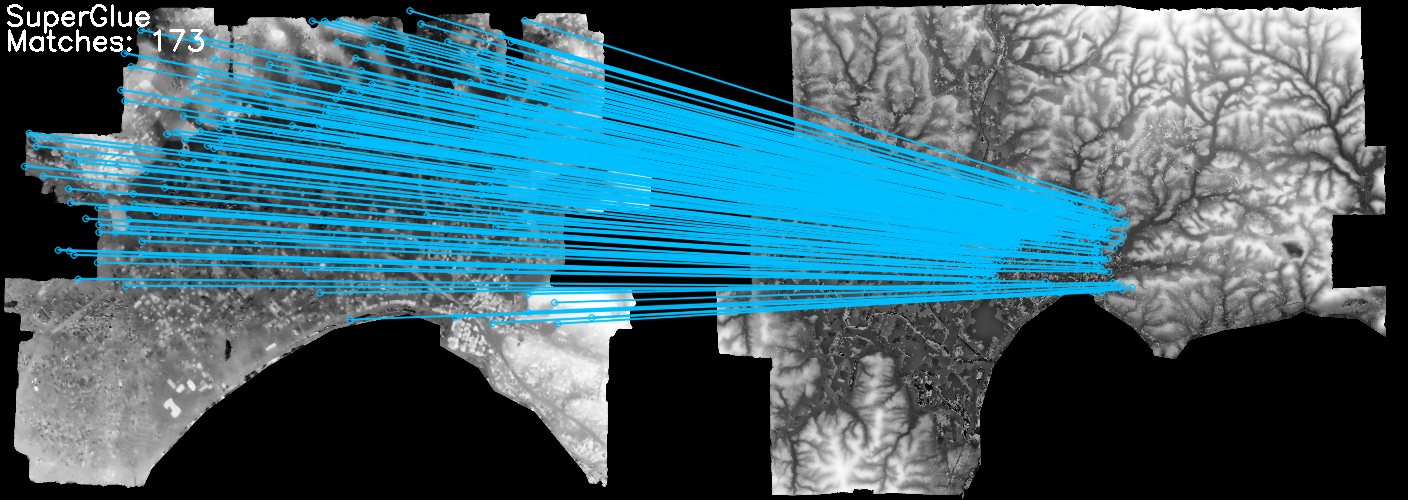
\includegraphics[width=6.8cm]{images/Chapitre3/Homol-SubPatch_R270-2DRANSAC_MEC-Malt_Tapas_1954_MEC-Malt_2014.png}
            \end{minipage}%
        }
        \caption{Result of matching DSMs of Fr{\'e}jus 1954 and 2014.}
        \label{Match result}
    \end{center}
\end{figure*} 



\begin{figure*}[htbp]
    \begin{center}
        \subfigure[Image pairs]{
            \begin{minipage}[t]{0.65\linewidth}
                \centering
                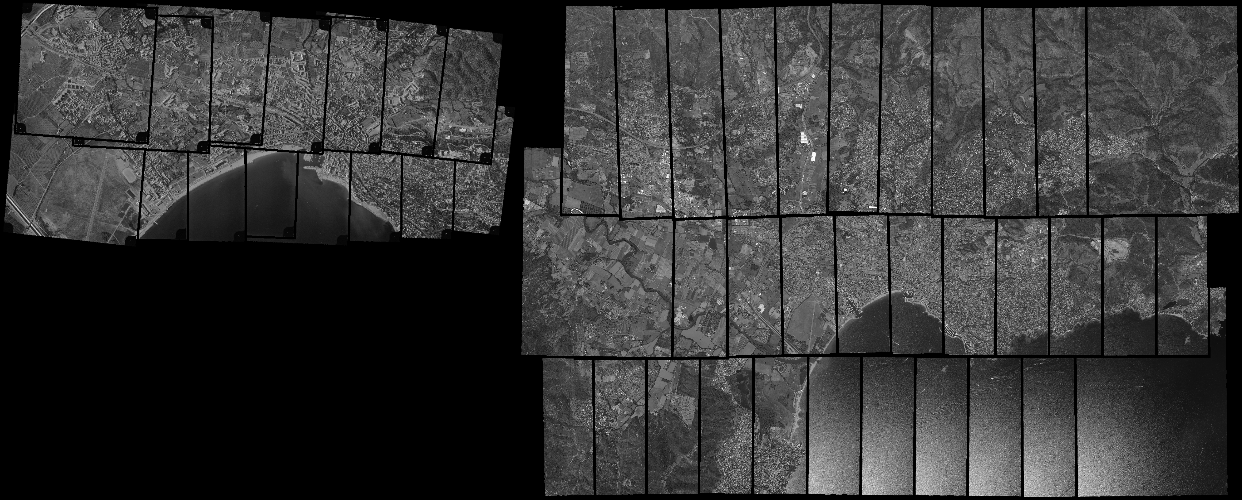
\includegraphics[width=8.1cm]{images/Chapitre3/Pseudo-Ortho-MEC-Malt_Tapas_1966_Ortho-MEC-Malt_2014.png}
            \end{minipage}%
        }
        \subfigure[Match number (\textit{ImgPairs})]{
            \begin{minipage}[t]{0.3\linewidth}
                \centering
                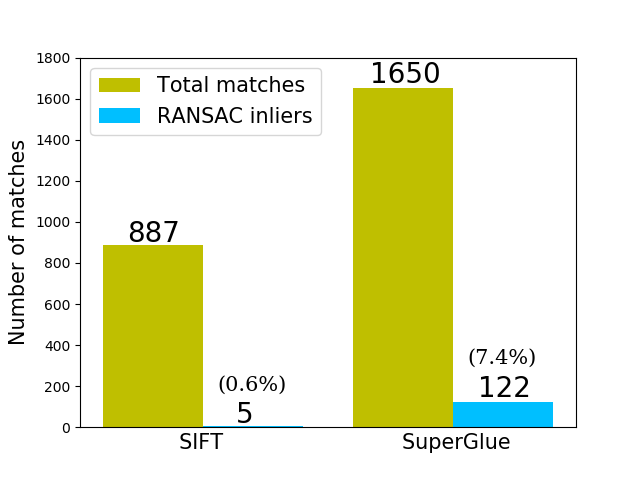
\includegraphics[width=4.8cm]{images/Chapitre3/PlotCurves_Pseudo-Ortho-MEC-Malt_Tapas_1966_Ortho-MEC-Malt_2014.png}
            \end{minipage}%
        }
        \subfigure[$SIFT_{ImgPairs}^{RANSAC Inliers}$]{
            \begin{minipage}[t]{0.48\linewidth}
                \centering
                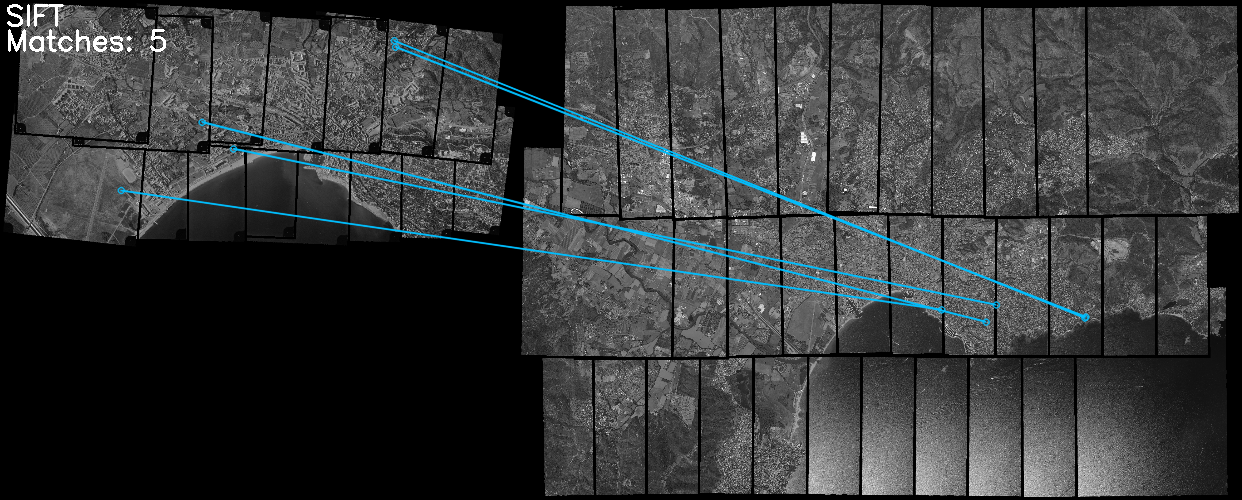
\includegraphics[width=6cm]{images/Chapitre3/Pseudo-Homol-SIFT2Step_1966-2014-Rough-2DRANSAC-GlobalR3D-PileImg_Ortho-MEC-Malt_Tapas_1966_Ortho-MEC-Malt_2014.png}
            \end{minipage}%
        }
        \subfigure[$SuperGlue_{ImgPairs}^{RANSAC Inliers}$]{
            \begin{minipage}[t]{0.48\linewidth}
                \centering
                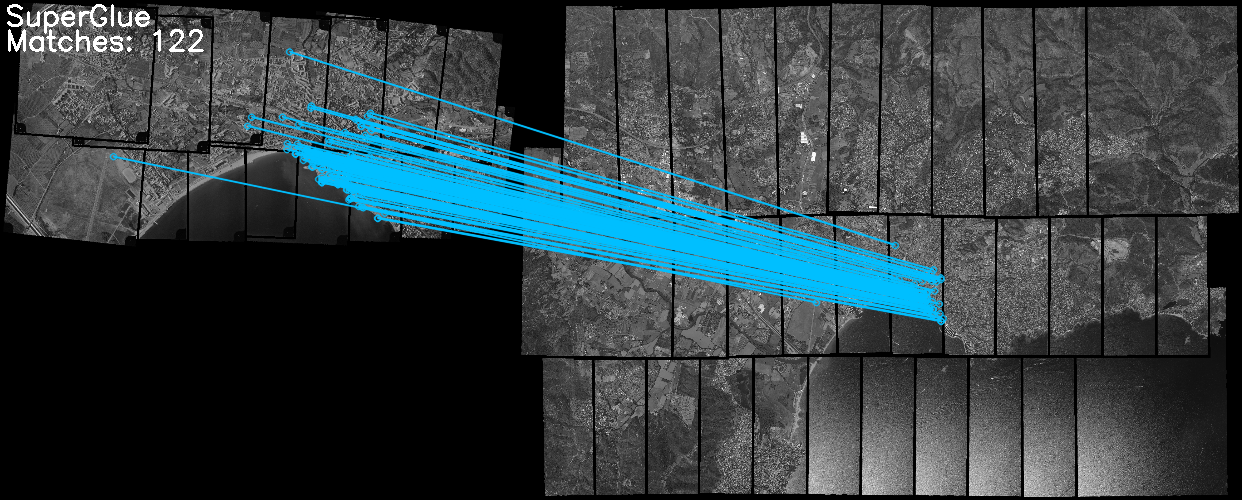
\includegraphics[width=6cm]{images/Chapitre3/Pseudo-Homol-SuperGlue_1966-2014-GlobalR3D-PileImg_Ortho-MEC-Malt_Tapas_1966_Ortho-MEC-Malt_2014.png}
            \end{minipage}%
        }
        \caption{Result of matching image pairs of Fr{\'e}jus 1966 and 2014.}
        \label{Match result}
    \end{center}
\end{figure*} 


\begin{figure*}[htbp]
    \begin{center}
        \subfigure[Orthophotos]{
            \begin{minipage}[t]{0.65\linewidth}
                \centering
                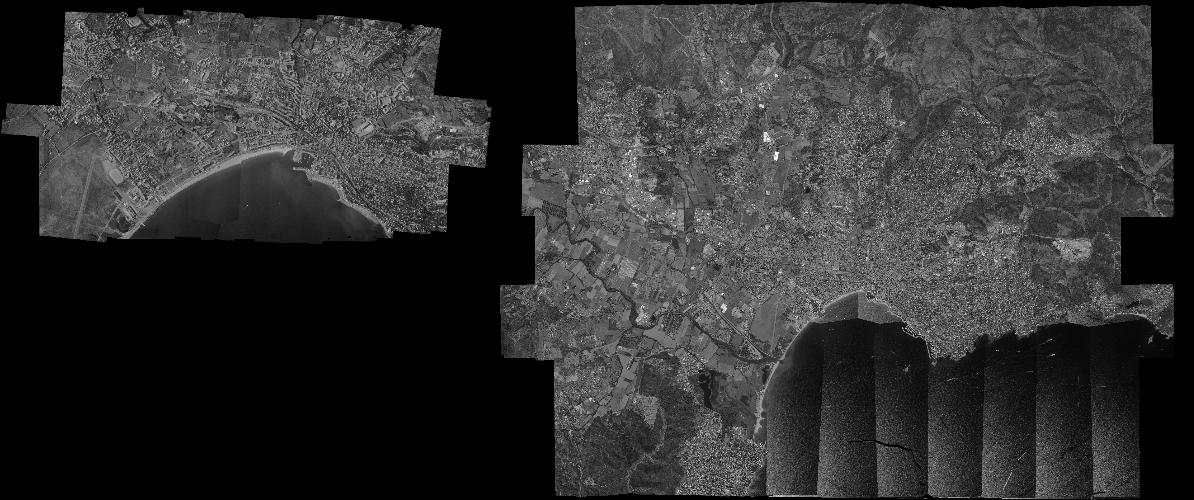
\includegraphics[width=8.1cm]{images/Chapitre3/Ortho-MEC-Malt_Tapas_1966_Ortho-MEC-Malt_2014.png}
            \end{minipage}%
        }
        \subfigure[Match number (\textit{Ortho})]{
            \begin{minipage}[t]{0.3\linewidth}
                \centering
                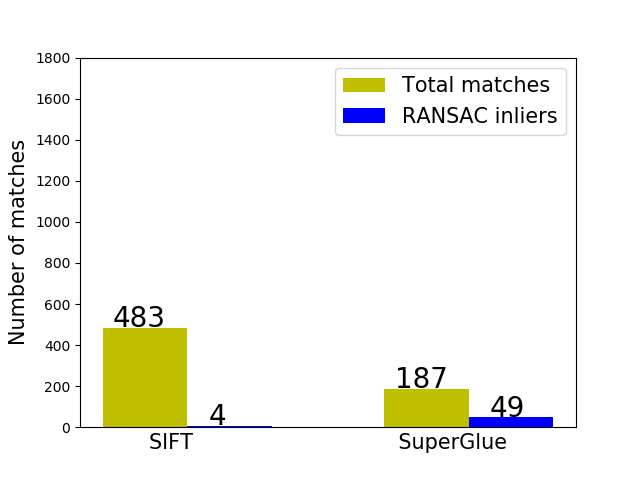
\includegraphics[width=4.8cm]{images/Chapitre3/PlotCurves_Ortho-MEC-Malt_Tapas_1966_Ortho-MEC-Malt_2014.png}
            \end{minipage}%
        }
        \subfigure[$SIFT_{Ortho}^{RANSAC Inliers}$]{
            \begin{minipage}[t]{0.48\linewidth}
                \centering
                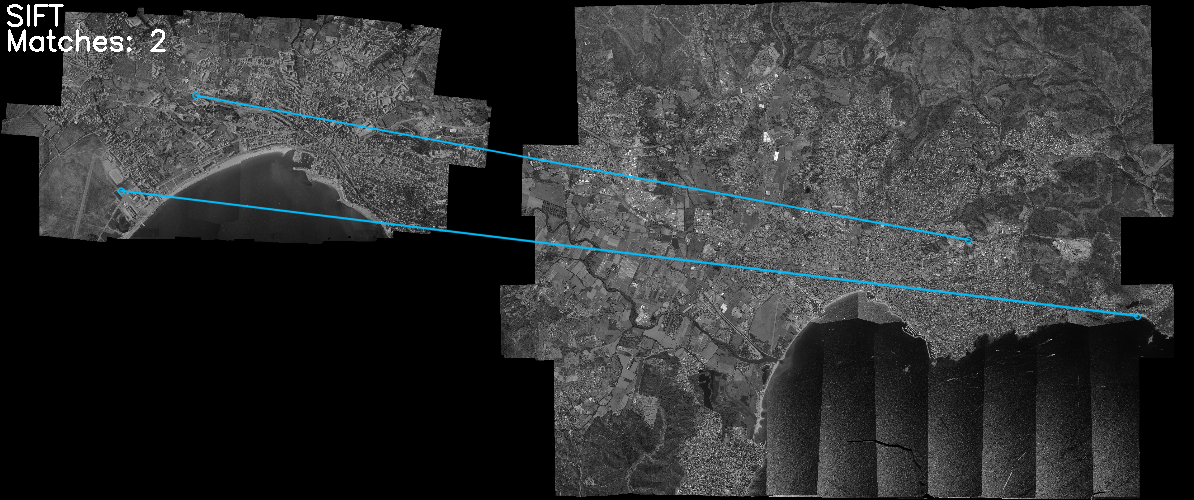
\includegraphics[width=6cm]{images/Chapitre3/Homol-SIFT-2DRANSAC_Ortho-MEC-Malt_Tapas_1966_Ortho-MEC-Malt_2014.png}
            \end{minipage}%
        }
        \subfigure[$SuperGlue_{Ortho}^{RANSAC Inliers}$]{
            \begin{minipage}[t]{0.48\linewidth}
                \centering
                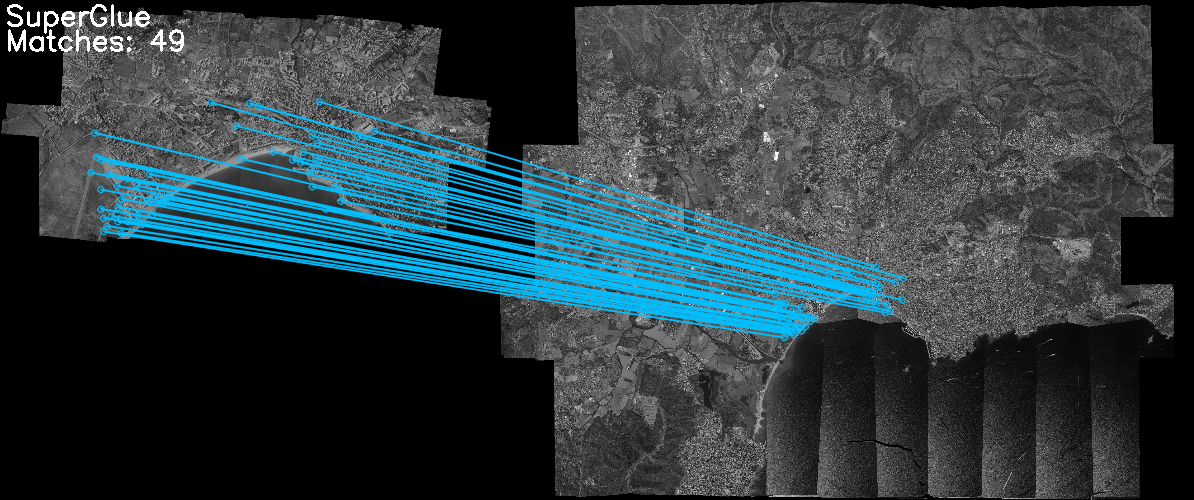
\includegraphics[width=6cm]{images/Chapitre3/Homol-SubPatch_R270-2DRANSAC_Ortho-MEC-Malt_Tapas_1966_Ortho-MEC-Malt_2014.png}
            \end{minipage}%
        }
        \caption{Result of matching orthophotos of Fr{\'e}jus 1966 and 2014.}
        \label{Match result}
    \end{center}
\end{figure*} 

\begin{figure*}[htbp]
    \begin{center}
        \subfigure[DSMs]{
            \begin{minipage}[t]{0.65\linewidth}
                \centering
                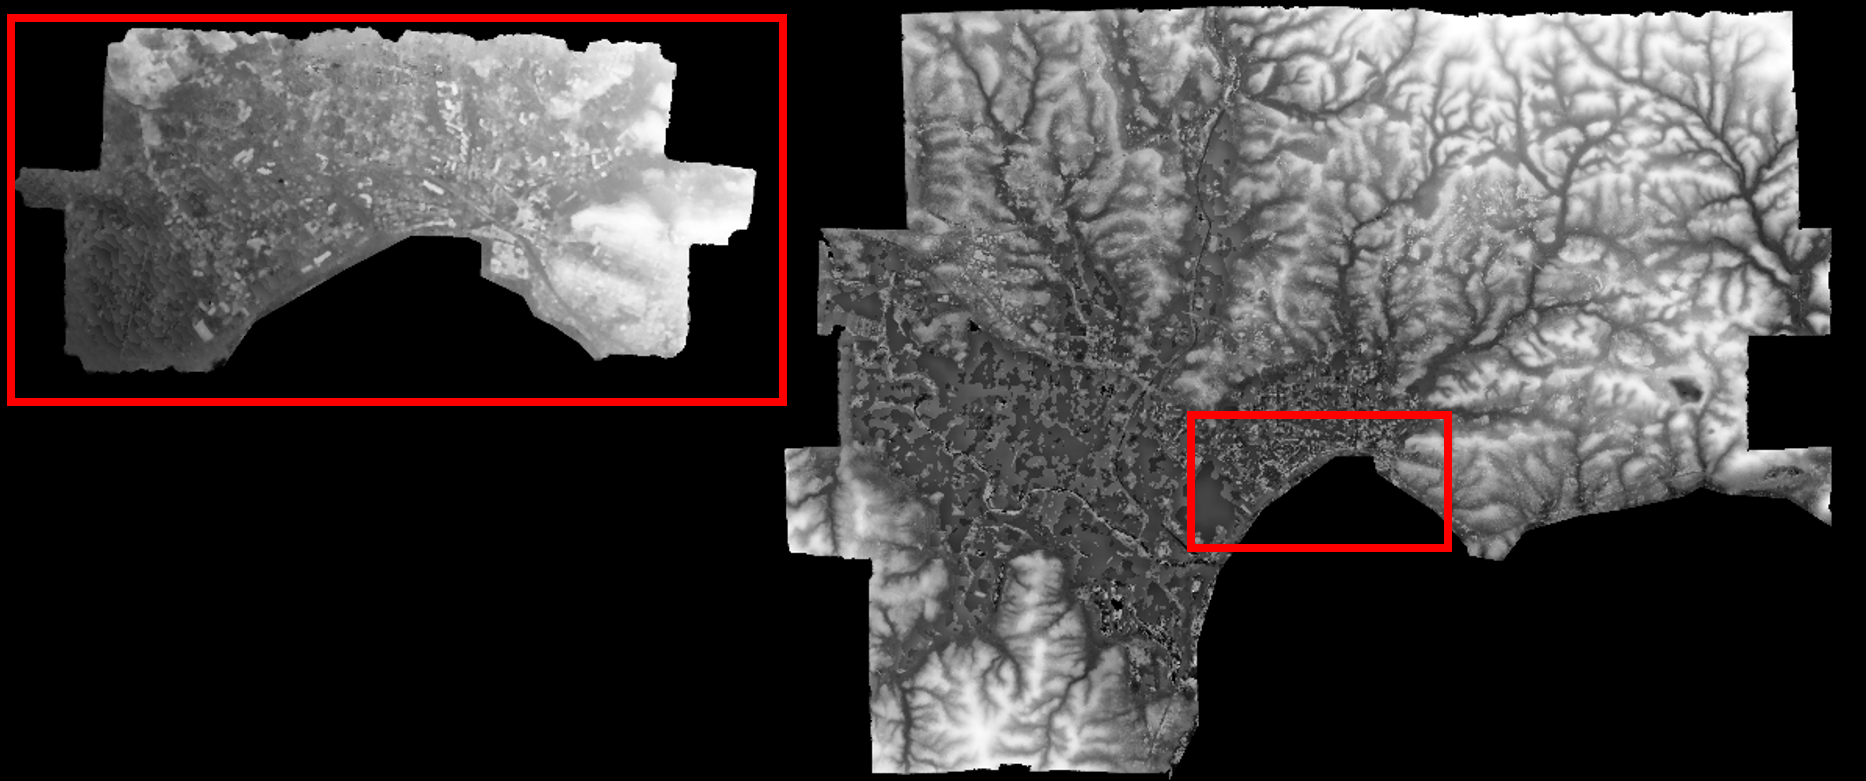
\includegraphics[width=8.1cm]{images/Chapitre3/MEC-Malt_Tapas_1966_MEC-Malt_2014.png}
            \end{minipage}%
        }
        \subfigure[Match number (\textit{DSM})]{
            \begin{minipage}[t]{0.3\linewidth}
                \centering
                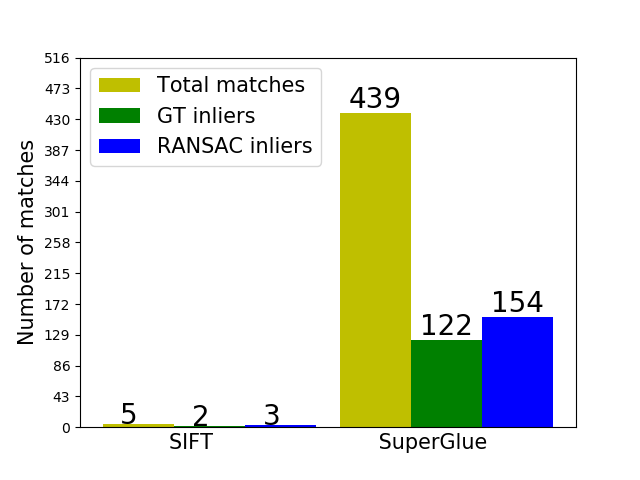
\includegraphics[width=4.8cm]{images/Chapitre3/PlotCurves_MEC-Malt_Tapas_1966_MEC-Malt_2014.png}
            \end{minipage}%
        }
        \subfigure[$SIFT_{DSM}^{RANSAC Inliers}$]{
            \begin{minipage}[t]{0.48\linewidth}
                \centering
                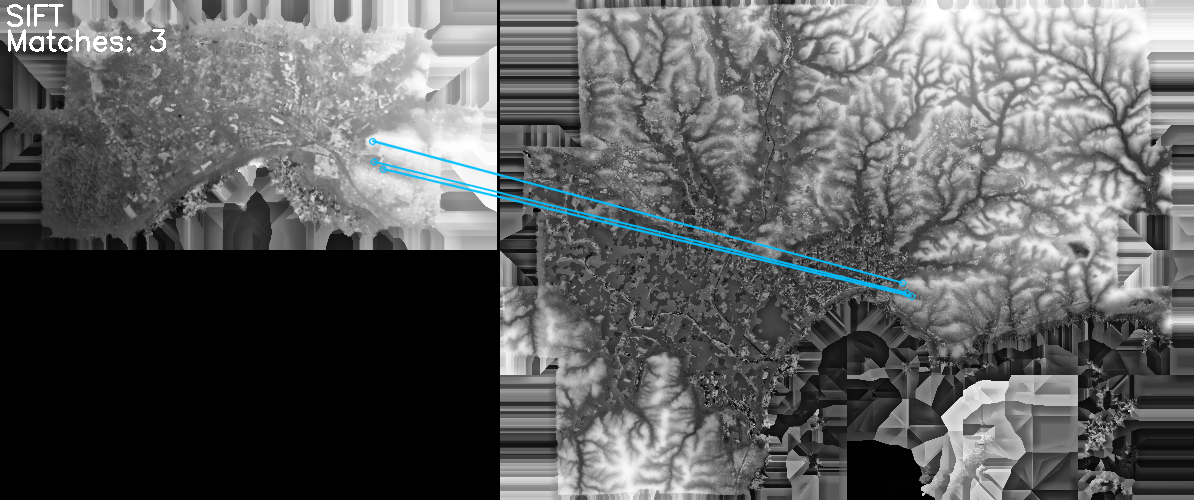
\includegraphics[width=6cm]{images/Chapitre3/Homol-SIFT-2DRANSAC_MEC-Malt_Tapas_1966_MEC-Malt_2014.png}
            \end{minipage}%
        }
        \subfigure[$SuperGlue_{DSM}^{RANSAC Inliers}$]{
            \begin{minipage}[t]{0.48\linewidth}
                \centering
                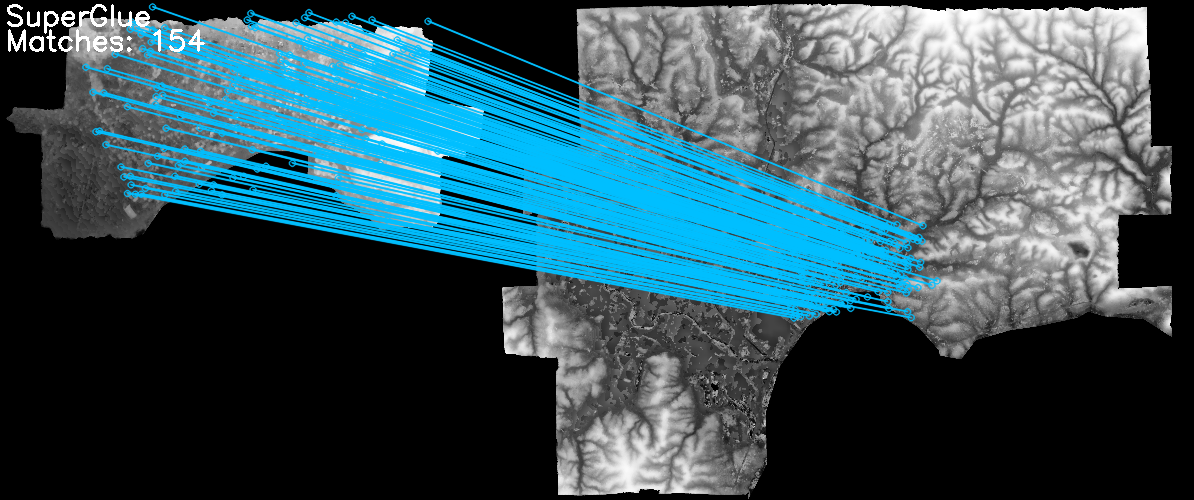
\includegraphics[width=6cm]{images/Chapitre3/Homol-SubPatch_R270-2DRANSAC_MEC-Malt_Tapas_1966_MEC-Malt_2014.png}
            \end{minipage}%
        }
        \caption{Result of matching DSMs of Fr{\'e}jus 1966 and 2014.}
        \label{Match result}
    \end{center}
\end{figure*} 


\begin{figure*}[htbp]
    \begin{center}
        \subfigure[Image pairs]{
            \begin{minipage}[t]{0.6\linewidth}
                \centering
                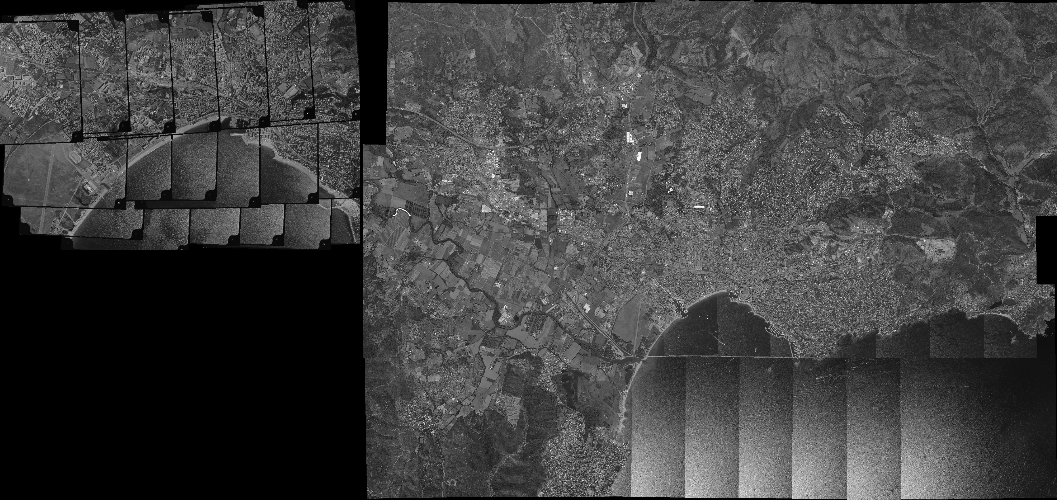
\includegraphics[width=7.8cm]{images/Chapitre3/Pseudo-Ortho-MEC-Malt_Tapas_1970_Ortho-MEC-Malt_2014.png}
            \end{minipage}%
        }
        \subfigure[Match number (\textit{ImgPairs})]{
            \begin{minipage}[t]{0.35\linewidth}
                \centering
                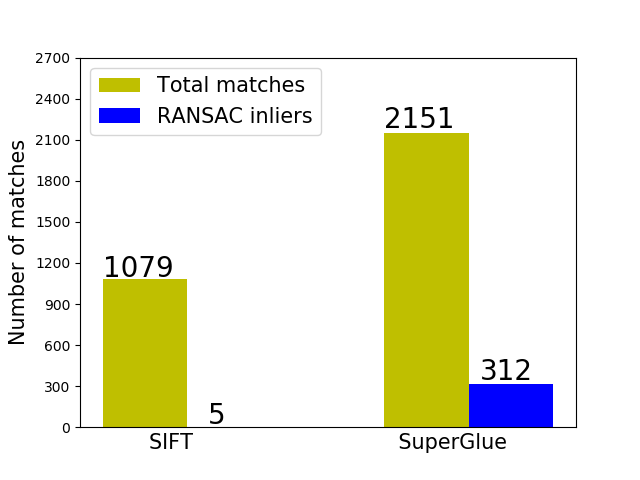
\includegraphics[width=4.8cm]{images/Chapitre3/PlotCurves_Pseudo-Ortho-MEC-Malt_Tapas_1970_Ortho-MEC-Malt_2014.png}
            \end{minipage}%
        }
        \subfigure[$SIFT_{ImgPairs}^{RANSAC Inliers}$]{
            \begin{minipage}[t]{0.48\linewidth}
                \centering
                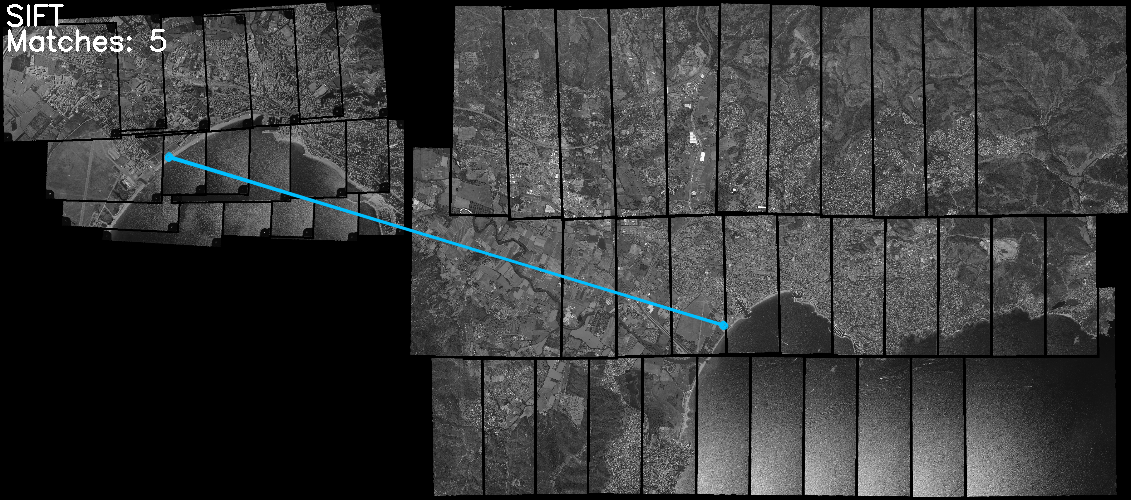
\includegraphics[width=6cm]{images/Chapitre3/Pseudo-Homol-SIFT2Step_1970-2014-Rough-2DRANSAC-GlobalR3D-PileImg_Ortho-MEC-Malt_Tapas_1970_Ortho-MEC-Malt_2014.png}
            \end{minipage}%
        }
        \subfigure[$SuperGlue_{ImgPairs}^{RANSAC Inliers}$]{
            \begin{minipage}[t]{0.48\linewidth}
                \centering
                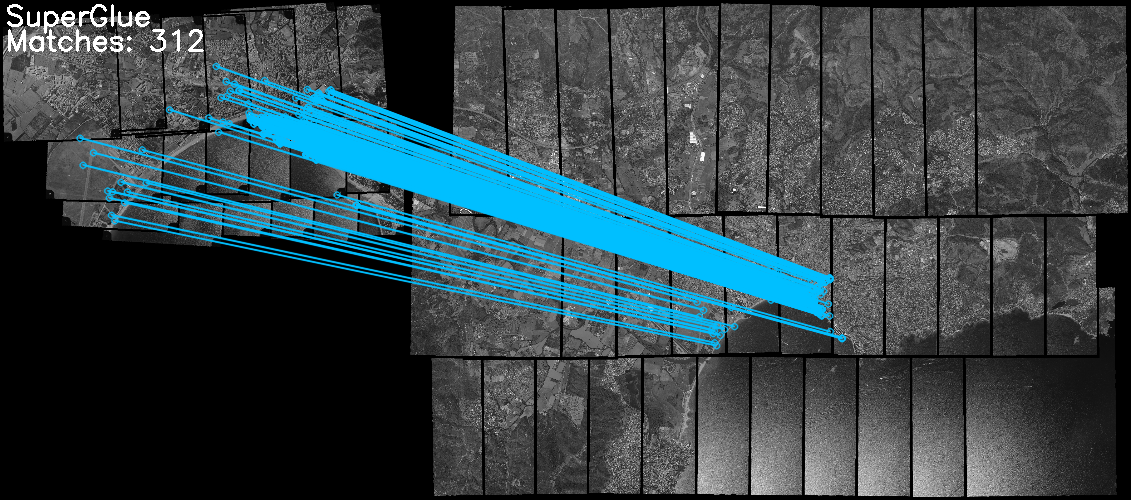
\includegraphics[width=6cm]{images/Chapitre3/Pseudo-Homol-SuperGlue_1970-2014-GlobalR3D-PileImg_Ortho-MEC-Malt_Tapas_1970_Ortho-MEC-Malt_2014.png}
            \end{minipage}%
        }
        \caption{Result of matching image pairs of Fr{\'e}jus 1970 and 2014.}
        \label{Match result}
    \end{center}
\end{figure*} 

\begin{figure*}[htbp]
    \begin{center}
        \subfigure[Orthophotos]{
            \begin{minipage}[t]{0.6\linewidth}
                \centering
                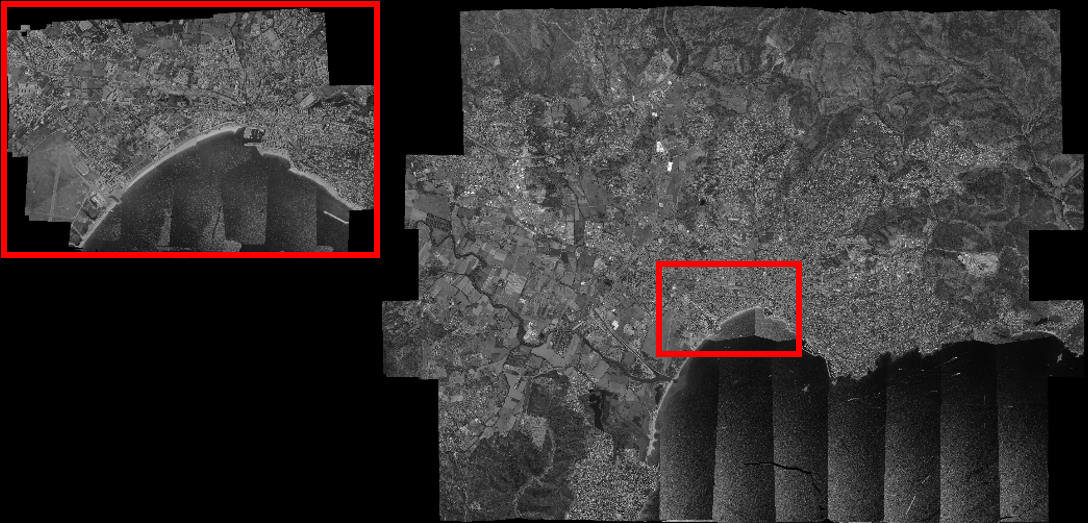
\includegraphics[width=7.8cm]{images/Chapitre3/Ortho-MEC-Malt_Tapas_1970_Ortho-MEC-Malt_2014.png}
            \end{minipage}%
        }
        \subfigure[Match number (\textit{Ortho})]{
            \begin{minipage}[t]{0.35\linewidth}
                \centering
                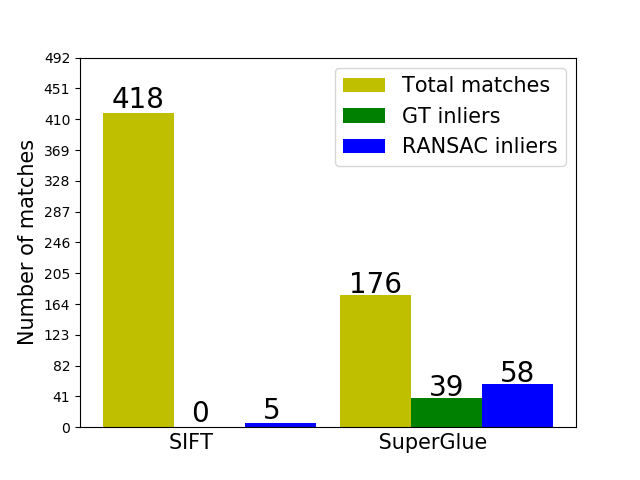
\includegraphics[width=4.8cm]{images/Chapitre3/PlotCurves_Ortho-MEC-Malt_Tapas_1970_Ortho-MEC-Malt_2014.png}
            \end{minipage}%
        }
        \subfigure[$SIFT_{Ortho}^{RANSAC Inliers}$]{
            \begin{minipage}[t]{0.48\linewidth}
                \centering
                \includegraphics[width=6cm]{images/Chapitre3/Homol-SIFT-2DRANSAC_Ortho-MEC-Malt_Tapas_1970_Ortho-MEC-Malt_2014.png}
            \end{minipage}%
        }
        \subfigure[$SuperGlue_{Ortho}^{RANSAC Inliers}$]{
            \begin{minipage}[t]{0.48\linewidth}
                \centering
                \includegraphics[width=6cm]{images/Chapitre3/Homol-SubPatch_R270-2DRANSAC_Ortho-MEC-Malt_Tapas_1970_Ortho-MEC-Malt_2014.png}
            \end{minipage}%
        }
        \caption{Result of matching orthophotos of Fr{\'e}jus 1970 and 2014.}
        \label{Match result}
    \end{center}
\end{figure*} 

\begin{figure*}[htbp]
    \begin{center}
        \subfigure[DSMs]{
            \begin{minipage}[t]{0.6\linewidth}
                \centering
                \includegraphics[width=7.8cm]{images/Chapitre3/MEC-Malt_Tapas_1970_MEC-Malt_2014.png}
            \end{minipage}%
        }
        \subfigure[Match number (\textit{DSM})]{
            \begin{minipage}[t]{0.35\linewidth}
                \centering
                \includegraphics[width=4.8cm]{images/Chapitre3/PlotCurves_MEC-Malt_Tapas_1970_MEC-Malt_2014.png}
            \end{minipage}%
        }
        \subfigure[$SIFT_{DSM}^{RANSAC Inliers}$]{
            \begin{minipage}[t]{0.48\linewidth}
                \centering
                \includegraphics[width=6cm]{images/Chapitre3/Homol-SIFT-2DRANSAC_MEC-Malt_Tapas_1970_MEC-Malt_2014.png}
            \end{minipage}%
        }
        \subfigure[$SuperGlue_{DSM}^{RANSAC Inliers}$]{
            \begin{minipage}[t]{0.48\linewidth}
                \centering
                \includegraphics[width=6cm]{images/Chapitre3/Homol-SubPatch_R270-2DRANSAC_MEC-Malt_Tapas_1970_MEC-Malt_2014.png}
            \end{minipage}%
        }
        \caption{Result of matching DSMs of Fr{\'e}jus 1970 and 2014.}
        \label{Match result}
    \end{center}
\end{figure*} 


%%%%%%%%%%%%%%%%%%%%%%%%%%%%%%%%%%%%%%Pezenas
\begin{figure*}[htbp]
    \begin{center}
        \subfigure[Image pairs]{
            \begin{minipage}[t]{0.65\linewidth}
                \centering
                \includegraphics[width=8.8cm]{images/Chapitre3/Pseudo-Ortho-MEC-Malt_Tapas_1971_Ortho-MEC-Malt_2015.png}
            \end{minipage}%
        }
        \subfigure[Match number (\textit{ImgPairs})]{
            \begin{minipage}[t]{0.3\linewidth}
                \centering
                \includegraphics[width=4.8cm]{images/Chapitre3/PlotCurves_Pseudo-Ortho-MEC-Malt_Tapas_1971_Ortho-MEC-Malt_2015.png}
            \end{minipage}%
        }
        \subfigure[$SIFT_{ImgPairs}^{RANSAC Inliers}$]{
            \begin{minipage}[t]{0.48\linewidth}
                \centering
                \includegraphics[width=6.8cm]{images/Chapitre3/Pseudo-Homol-SIFT2Step_1971-2015-Rough-2DRANSAC-GlobalR3D-PileImg_Ortho-MEC-Malt_Tapas_1971_Ortho-MEC-Malt_2015.png}
            \end{minipage}%
        }
        \subfigure[$SuperGlue_{ImgPairs}^{RANSAC Inliers}$]{
            \begin{minipage}[t]{0.48\linewidth}
                \centering
                \includegraphics[width=6.8cm]{images/Chapitre3/Pseudo-Homol-SuperGlue_1971-2015-GlobalR3D-PileImg_Ortho-MEC-Malt_Tapas_1971_Ortho-MEC-Malt_2015.png}
            \end{minipage}%
        }
        \caption{Result of matching image pairs of Pezenas 1971 and 2015.}
        \label{Match result}
    \end{center}
\end{figure*} 



\begin{figure*}[htbp]
    \begin{center}
        \subfigure[Orthophotos]{
            \begin{minipage}[t]{0.65\linewidth}
                \centering
                \includegraphics[width=8.8cm]{images/Chapitre3/Ortho-MEC-Malt_Tapas_1971_Ortho-MEC-Malt_2015.png}
            \end{minipage}%
        }
        \subfigure[Match number (\textit{Ortho})]{
            \begin{minipage}[t]{0.3\linewidth}
                \centering
                \includegraphics[width=4.8cm]{images/Chapitre3/PlotCurves_Ortho-MEC-Malt_Tapas_1971_Ortho-MEC-Malt_2015.png}
            \end{minipage}%
        }
        \subfigure[$SIFT_{Ortho}^{RANSAC Inliers}$]{
            \begin{minipage}[t]{0.48\linewidth}
                \centering
                \includegraphics[width=6.8cm]{images/Chapitre3/Homol-SIFT-2DRANSAC_Ortho-MEC-Malt_Tapas_1971_Ortho-MEC-Malt_2015.png}
            \end{minipage}%
        }
        \subfigure[$SuperGlue_{Ortho}^{RANSAC Inliers}$]{
            \begin{minipage}[t]{0.48\linewidth}
                \centering
                \includegraphics[width=6.8cm]{images/Chapitre3/Homol-SubPatch_R270-2DRANSAC_Ortho-MEC-Malt_Tapas_1971_Ortho-MEC-Malt_2015.png}
            \end{minipage}%
        }
        \caption{Result of matching orthophotos of Pezenas 1971 and 2015.}
        \label{Match result}
    \end{center}
\end{figure*} 


\begin{figure*}[htbp]
    \begin{center}
        \subfigure[DSMs]{
            \begin{minipage}[t]{0.65\linewidth}
                \centering
                \includegraphics[width=8.8cm]{images/Chapitre3/MEC-Malt_Tapas_1971_MEC-Malt_2015.png}
            \end{minipage}%
        }
        \subfigure[Match number (\textit{DSM})]{
            \begin{minipage}[t]{0.3\linewidth}
                \centering
                \includegraphics[width=4.8cm]{images/Chapitre3/PlotCurves_MEC-Malt_Tapas_1971_MEC-Malt_2015.png}
            \end{minipage}%
        }
        \subfigure[$SIFT_{DSM}^{RANSAC Inliers}$]{
            \begin{minipage}[t]{0.48\linewidth}
                \centering
                \includegraphics[width=6.8cm]{images/Chapitre3/Homol-SIFT-2DRANSAC_MEC-Malt_Tapas_1971_MEC-Malt_2015.png}
            \end{minipage}%
        }
        \subfigure[$SuperGlue_{DSM}^{RANSAC Inliers}$]{
            \begin{minipage}[t]{0.48\linewidth}
                \centering
                \includegraphics[width=6.8cm]{images/Chapitre3/Homol-SubPatch_R270-2DRANSAC_MEC-Malt_Tapas_1971_MEC-Malt_2015.png}
            \end{minipage}%
        }
        \caption{Result of matching DSMs of Pezenas 1971 and 2015.}
        \label{Match result}
    \end{center}
\end{figure*} 



\begin{figure*}[htbp]
    \begin{center}
        \subfigure[Image pairs]{
            \begin{minipage}[t]{0.65\linewidth}
                \centering
                \includegraphics[width=8.1cm]{images/Chapitre3/Pseudo-Ortho-MEC-Malt_Tapas_1981_Ortho-MEC-Malt_2015.png}
            \end{minipage}%
        }
        \subfigure[Match number (\textit{ImgPairs})]{
            \begin{minipage}[t]{0.3\linewidth}
                \centering
                \includegraphics[width=4.8cm]{images/Chapitre3/PlotCurves_Pseudo-Ortho-MEC-Malt_Tapas_1981_Ortho-MEC-Malt_2015.png}
            \end{minipage}%
        }
        \subfigure[$SIFT_{ImgPairs}^{RANSAC Inliers}$]{
            \begin{minipage}[t]{0.48\linewidth}
                \centering
                \includegraphics[width=6cm]{images/Chapitre3/Pseudo-Homol-SIFT2Step_1981-2015-Rough-2DRANSAC-GlobalR3D-PileImg_Ortho-MEC-Malt_Tapas_1981_Ortho-MEC-Malt_2015.png}
            \end{minipage}%
        }
        \subfigure[$SuperGlue_{ImgPairs}^{RANSAC Inliers}$]{
            \begin{minipage}[t]{0.48\linewidth}
                \centering
                \includegraphics[width=6cm]{images/Chapitre3/Pseudo-Homol-SuperGlue_1981-2015-GlobalR3D-PileImg_Ortho-MEC-Malt_Tapas_1981_Ortho-MEC-Malt_2015.png}
            \end{minipage}%
        }
        \caption{Result of matching image pairs of Pezenas 1981 and 2015.}
        \label{Match result}
    \end{center}
\end{figure*} 


\begin{figure*}[htbp]
    \begin{center}
        \subfigure[Orthophotos]{
            \begin{minipage}[t]{0.65\linewidth}
                \centering
                \includegraphics[width=8.1cm]{images/Chapitre3/Ortho-MEC-Malt_Tapas_1981_Ortho-MEC-Malt_2015.png}
            \end{minipage}%
        }
        \subfigure[Match number (\textit{Ortho})]{
            \begin{minipage}[t]{0.3\linewidth}
                \centering
                \includegraphics[width=4.8cm]{images/Chapitre3/PlotCurves_Ortho-MEC-Malt_Tapas_1981_Ortho-MEC-Malt_2015.png}
            \end{minipage}%
        }
        \subfigure[$SIFT_{Ortho}^{RANSAC Inliers}$]{
            \begin{minipage}[t]{0.48\linewidth}
                \centering
                \includegraphics[width=6cm]{images/Chapitre3/Homol-SIFT-2DRANSAC_Ortho-MEC-Malt_Tapas_1981_Ortho-MEC-Malt_2015.png}
            \end{minipage}%
        }
        \subfigure[$SuperGlue_{Ortho}^{RANSAC Inliers}$]{
            \begin{minipage}[t]{0.48\linewidth}
                \centering
                \includegraphics[width=6cm]{images/Chapitre3/Homol-SubPatch_R90-2DRANSAC_Ortho-MEC-Malt_Tapas_1981_Ortho-MEC-Malt_2015.png}
            \end{minipage}%
        }
        \caption{Result of matching orthophotos of Pezenas 1981 and 2015.}
        \label{Match result}
    \end{center}
\end{figure*} 

\begin{figure*}[htbp]
    \begin{center}
        \subfigure[DSMs]{
            \begin{minipage}[t]{0.65\linewidth}
                \centering
                \includegraphics[width=8.1cm]{images/Chapitre3/MEC-Malt_Tapas_1981_MEC-Malt_2015.png}
            \end{minipage}%
        }
        \subfigure[Match number (\textit{DSM})]{
            \begin{minipage}[t]{0.3\linewidth}
                \centering
                \includegraphics[width=4.8cm]{images/Chapitre3/PlotCurves_MEC-Malt_Tapas_1981_MEC-Malt_2015.png}
            \end{minipage}%
        }
        \subfigure[$SIFT_{DSM}^{RANSAC Inliers}$]{
            \begin{minipage}[t]{0.48\linewidth}
                \centering
                \includegraphics[width=6cm]{images/Chapitre3/Homol-SIFT-2DRANSAC_MEC-Malt_Tapas_1981_MEC-Malt_2015.png}
            \end{minipage}%
        }
        \subfigure[$SuperGlue_{DSM}^{RANSAC Inliers}$]{
            \begin{minipage}[t]{0.48\linewidth}
                \centering
                \includegraphics[width=6cm]{images/Chapitre3/Homol-SubPatch_R90-2DRANSAC_MEC-Malt_Tapas_1981_MEC-Malt_2015.png}
            \end{minipage}%
        }
        \caption{Result of matching DSMs of Pezenas 1981 and 2015.}
        \label{Match result}
    \end{center}
\end{figure*} 


%%%%%%%%%%%%%%%%%%%%%%%%%%%%%%%%%%%%%%Kobe

\begin{figure*}[htbp]
    \begin{center}
        \subfigure[Image pairs]{
            \begin{minipage}[t]{0.45\linewidth}
                \centering
                \includegraphics[width=5.5cm]{images/Chapitre3/Pseudo-Ortho-MEC-Malt_Tapas_1991_Ortho-MEC-Malt_Tapas_1994.png}
            \end{minipage}%
        }
        \subfigure[Match number (\textit{ImgPairs})]{
            \begin{minipage}[t]{0.35\linewidth}
                \centering
                \includegraphics[width=4.8cm]{images/Chapitre3/PlotCurves_Pseudo-Ortho-MEC-Malt_Tapas_1991_Ortho-MEC-Malt_Tapas_1994.png}
            \end{minipage}%
        }   
        \subfigure[$SIFT_{ImgPairs}^{RANSAC Inliers}$]{
            \begin{minipage}[t]{0.45\linewidth}
                \centering
                \includegraphics[width=5.5cm]{images/Chapitre3/Pseudo-Homol-SIFT2Step_1991-1994-Rough-2DRANSAC-GlobalR3D-PileImg_Ortho-MEC-Malt_Tapas_1991_Ortho-MEC-Malt_Tapas_1994.png}
            \end{minipage}%
        }
        \subfigure[$SuperGlue_{ImgPairs}^{RANSAC Inliers}$]{
            \begin{minipage}[t]{0.45\linewidth}
                \centering
                \includegraphics[width=5.5cm]{images/Chapitre3/Pseudo-Homol-SuperGlue_1991-1994-GlobalR3D-PileImg_Ortho-MEC-Malt_Tapas_1991_Ortho-MEC-Malt_Tapas_1994.png}
            \end{minipage}%
        }
        \caption{Result of matching image pairs of Kobe 1991 and 1995.}
        \label{Match result}
    \end{center}
\end{figure*} 

\begin{figure*}[htbp]
    \begin{center}
        \subfigure[Orthophotos]{
            \begin{minipage}[t]{0.45\linewidth}
                \centering
                \includegraphics[width=5.5cm]{images/Chapitre3/Ortho-MEC-Malt_Tapas_1991_Ortho-MEC-Malt_Tapas_1994.png}
            \end{minipage}%
        }
        \subfigure[Match number (\textit{Ortho})]{
            \begin{minipage}[t]{0.35\linewidth}
                \centering
                \includegraphics[width=4.8cm]{images/Chapitre3/PlotCurves_Ortho-MEC-Malt_Tapas_1991_Ortho-MEC-Malt_Tapas_1994.png}
            \end{minipage}%
        }   
        \subfigure[$SIFT_{Ortho}^{RANSAC Inliers}$]{
            \begin{minipage}[t]{0.45\linewidth}
                \centering
                \includegraphics[width=5.5cm]{images/Chapitre3/Homol-SIFT-2DRANSAC_Ortho-MEC-Malt_Tapas_1991_Ortho-MEC-Malt_Tapas_1994.png}
            \end{minipage}%
        }
        \subfigure[$SuperGlue_{Ortho}^{RANSAC Inliers}$]{
            \begin{minipage}[t]{0.45\linewidth}
                \centering
                \includegraphics[width=5.5cm]{images/Chapitre3/Homol-SubPatch-2DRANSAC_Ortho-MEC-Malt_Tapas_1991_Ortho-MEC-Malt_Tapas_1994.png}
            \end{minipage}%
        }
        \caption{Result of matching orthophotos of Kobe 1991 and 1995.}
        \label{Match result}
    \end{center}
\end{figure*} 

\begin{figure*}[htbp]
    \begin{center}
        \subfigure[DSMs]{
            \begin{minipage}[t]{0.45\linewidth}
                \centering
                \includegraphics[width=5.5cm]{images/Chapitre3/MEC-Malt_Tapas_1991_MEC-Malt_Tapas_1994.png}
            \end{minipage}%
        }
        \subfigure[Match number (\textit{DSM})]{
            \begin{minipage}[t]{0.35\linewidth}
                \centering
                \includegraphics[width=4.8cm]{images/Chapitre3/PlotCurves_MEC-Malt_Tapas_1991_MEC-Malt_Tapas_1994.png}
            \end{minipage}%
        }
        \subfigure[$SIFT_{DSM}^{RANSAC Inliers}$]{
            \begin{minipage}[t]{0.45\linewidth}
                \centering
                \includegraphics[width=5.5cm]{images/Chapitre3/Homol-SIFT-2DRANSAC_MEC-Malt_Tapas_1991_MEC-Malt_Tapas_1994.png}
            \end{minipage}%
        }
        \subfigure[$SuperGlue_{DSM}^{RANSAC Inliers}$]{
            \begin{minipage}[t]{0.45\linewidth}
                \centering
                \includegraphics[width=5.5cm]{images/Chapitre3/Homol-SubPatch-2DRANSAC_MEC-Malt_Tapas_1991_MEC-Malt_Tapas_1994.png}
            \end{minipage}%
        }
        \caption{Result of matching DSMs of Kobe 1991 and 1995.}
        \label{Match result}
    \end{center}
\end{figure*} 

%As can be seen, 


\subsubsection{Ground check points}

\begin{table}%[H]
    \footnotesize
    \centering
    \begin{tabular}{|l|c|c|c|c|c|c|}\hline
        &\multicolumn{6}{c|}{$|\mu|$ [m]}\\\hline
        &\multicolumn{2}{c|}{ImgPairs} &\multicolumn{2}{c|}{Orthophoto} &\multicolumn{2}{c|}{DSM}\\\hline
        & SIFT & SuperGlue & SIFT & SuperGlue & SIFT & SuperGlue \\\hline\hline
        $Frejus_{2014}^{1954}$ & 1380.16 & 29.29 & / & 34.84 & / & \textbf{10.72}\\\hline
        $Frejus_{2014}^{1966}$ & 1686.56 & 18.15 & / & 11.98 & / & \textbf{10.43}\\\hline
        $Frejus_{2014}^{1970}$ & 997.83 & 11.09 & / & 16.87 & / & \textbf{10.23}\\\hline\hline

        $Frejus_{2014}^{1966}$ & 1686.56 & 18.15 & / & 11.98 & / & \textbf{10.43}\\\hline
$Frejus_{2014}^{1970}$ & 997.83 & 11.09 & / & 16.87 & / & \textbf{10.23}\\\hline\hline

        $Kobe_{1994}^{1991}$ & / & \textbf{2.02} & / & 3.40 & 2.78 & 4.03 \\\hline
\end{tabular}
    \caption{Accuracy of 6 sets of co-registered orientations resulting from 6 methods, evaluated on 3 check points uniformly distributed in the block. Absolute average value $|\mu|$ is displayed for each method.}
    \label{CheckptAcuracy}
\end{table}

\subsubsection{DoD}


\begin{figure*}[htbp]
    \begin{center}
        \subfigure[DoD$_{Frejus1954}^{ImgPairs}$]{
            \begin{minipage}[t]{0.31\linewidth}
                \centering
                %left, lower, right, up
                \includegraphics[width=4.2cm,trim=550 60 230 200,clip]{images/Chapitre3/DoD1954R3D.png}
            \end{minipage}%
        }
        \subfigure[DoD$_{Frejus1954}^{Orthophoto}$]{
            \begin{minipage}[t]{0.31\linewidth}
                \centering
                \includegraphics[width=4.2cm,trim=550 60 230 200,clip]{images/Chapitre3/DoD1954Ortho.png}
            \end{minipage}%
        }
        \subfigure[DoD$_{Frejus1954}^{DSM}$]{
            \begin{minipage}[t]{0.31\linewidth}
                \centering
                \includegraphics[width=4.2cm,trim=550 60 230 200,clip]{images/Chapitre3/DoD1954DSM.png}
            \end{minipage}%
        }
        
        \subfigure[DoD$_{Frejus1966}^{ImgPairs}$]{
            \begin{minipage}[t]{0.31\linewidth}
                \centering
                %left, lower, right, up
                \includegraphics[width=4.2cm,trim=480 60 50 200,clip]{images/Chapitre3/DoD1966R3D.png}
            \end{minipage}%
        }
        \subfigure[DoD$_{Frejus1954}^{Orthophoto}$]{
            \begin{minipage}[t]{0.31\linewidth}
                \centering
                \includegraphics[width=4.2cm,trim=480 60 50 200,clip]{images/Chapitre3/DoD1966Ortho.png}
            \end{minipage}%
        }
        \subfigure[DoD$_{Frejus1966}^{DSM}$]{
            \begin{minipage}[t]{0.31\linewidth}
                \centering
                \includegraphics[width=4.2cm,trim=480 60 50 200,clip]{images/Chapitre3/DoD1966DSM.png}
            \end{minipage}%
        }
        
        \subfigure[DoD$_{Frejus1970}^{ImgPairs}$]{
            \begin{minipage}[t]{0.31\linewidth}
                \centering
                %left, lower, right, up
                \includegraphics[width=4.2cm,trim=480 110 50 200,clip]{images/Chapitre3/DoD1970R3D.png}
            \end{minipage}%
        }
        \subfigure[DoD$_{Frejus1970}^{Orthophoto}$]{
            \begin{minipage}[t]{0.31\linewidth}
                \centering
                \includegraphics[width=4.2cm,trim=480 110 50 200,clip]{images/Chapitre3/DoD1970Ortho.png}
            \end{minipage}%
        }
        \subfigure[DoD$_{Frejus1970}^{DSM}$]{
            \begin{minipage}[t]{0.31\linewidth}
                \centering
                \includegraphics[width=4.2cm,trim=480 110 50 200,clip]{images/Chapitre3/DoD1970DSM.png}
            \end{minipage}%
        }
        
        \subfigure[DoD legend]{
            \begin{minipage}[t]{1\linewidth}
                \centering
                \includegraphics[width=11cm]{images/Chapitre3/LegendDoD.png}
            \end{minipage}%
        }
        \caption{DoDs of SuperGlue on dataset Fr{\'e}jus.}
        \label{Frejus DoD of SuperGlue}
    \end{center}
\end{figure*} 

\begin{table}%[H]
    \footnotesize
    \centering
    \begin{tabular}{||l|c|c|c||}\hline
        &$\mu$ [m]&$\sigma$ [m]&$|\mu|$ [m]\\\hline\hline
        DoD$_{Frejus1954}^{ImgPairs}$ & 5.70 & 6.32 & 6.62\\
        DoD$_{Frejus1954}^{Orthophoto}$ & 2.19 & 6.46 & 4.55\\
        DoD$_{Frejus1954}^{DSM}$ & 2.07 & 4.87 & \textbf{3.83}\\\hline
        DoD$_{Frejus1966}^{ImgPairs}$ & -1.36 & 3.82 & 2.90\\
        DoD$_{Frejus1966}^{Orthophoto}$ & -0.37 & 4.22 & 3.01\\
        DoD$_{Frejus1966}^{DSM}$ & -0.46 & 3.77 & \textbf{2.68}\\\hline
        DoD$_{Frejus1970}^{ImgPairs}$ & -5.04 & 5.09 & 5.70\\
        DoD$_{Frejus1970}^{Orthophoto}$ & -2.63 & 5.18 & \textbf{4.39}\\
        DoD$_{Frejus1970}^{DSM}$ & -1.71 & 5.75 & 4.61\\\hline
        DoD$_{Kobe1991}^{ImgPairs}$ &-1.35 & 13.82 & \textbf{7.23}\\
        DoD$_{Kobe1991}^{Orthophoto}$ &-0.54 & 14.82 & 7.77\\
        DoD$_{Kobe1991}^{DSM}$ &-2.12 & 14.20 & 7.45\\\hline
    \end{tabular}
    \caption{Average value $\mu$, standard deviation $\sigma$, and absolute average value $|\mu|$ of all the DoDs in Figure~\ref{Frejus DoD of SuperGlue}.}
    \label{CheckptAcuracy}
\end{table}




\section{Conclusion}

\section{Discussion}

